% Dieser Text ist urheberrechtlich geschützt
% Er stellt einen Auszug eines von mir erstellten Referates dar
% und darf nicht gewerblich genutzt werden
% die private bzw. Studiums bezogen Nutzung ist frei
% Januar 2006
% Autor: Sascha Frank 
% Universität Freiburg 
% www.informatik.uni-freiburg.de/~frank/
% www.namsu.de/


\documentclass{beamer}
%%\usetheme{Warsaw-seahorse}
%\usepackage{german}
%\usepackage{ngerman}
\usepackage[utf8]{inputenc}
\usepackage[ngerman]{babel}
\usepackage{hyperref}

% Dia Abbildungen
\usepackage{tikz}

\usetheme{Warsaw}
\setbeamertemplate{headline}{}
%\usecolortheme{seahorse}
%\usefonttheme{serif}
\useinnertheme{rectangles}
%\usepackage{bookman}
\setbeamercovered{transparent}

%\setbeamertemplate{navigation symbols}{}
%\setbeamertemplate{footline}{}
%\setbeamertemplate{headline}{}


\usepackage{color} % used for comments
\usepackage{listings}%Quellcode

\usepackage{wrapfig}%floating elements

% Tabellen
\usepackage{array}
\usepackage{longtable}

\definecolor{Navy}{rgb}{0,0,0.5}
\definecolor{Gray}{gray}{0.5}
\definecolor{dunkelgrau}{rgb}{0.8,0.8,0.8}
\definecolor{hellgrau}{rgb}{0.95,0.95,0.95}
\definecolor{hellgrau2}{rgb}{0.93,0.93,0.93}
\definecolor{red}{rgb}{1,0, 0.2}
\definecolor{green}{rgb}{0,1,0.2}

\lstset {
  language=xml,
  basicstyle={\footnotesize\ttfamily},
  numbers=none,
  aboveskip=5mm,
  belowskip=5mm,
  showstringspaces=false,
  columns=flexible,
  keywordstyle={\bfseries\color{green}},
  commentstyle={\color{Red}\textit},
  stringstyle={\color{red}},
  frame=single,
  breaklines=true,
  breakatwhitespace=true,
  tabsize=4,
  morekeywords={xmlns:rdf, xmlns:rdfs, rdf:about, rdf:resource}  % <-- adding custom keywords
}
\lstset {
  language=sparql,
  basicstyle={\footnotesize\ttfamily},
  numbers=left,
  aboveskip=5mm,
  belowskip=5mm,
  showstringspaces=false,
  columns=flexible,
  keywordstyle={\bfseries\color{green}},
  commentstyle={\color{hellgrau}\textit},
  stringstyle={\color{red}},
  frame=single,
  breaklines=true,
  breakatwhitespace=true,
  tabsize=4,
  morekeywords={PREFIX, select, SELECT, where, WHERE, Filter, filter, FILTER}  % <-- adding custom keywords
}

% Fußnoten korrigieren:
\makeatletter
 \renewcommand\@makefntext[1]{%
  \setlength{\hangindent}{2em}
  \noindent
  \hb@xt@\hangindent{%
     \hss\@textsuperscript{\normalfont\@thefnmark}\hspace{.1em}}#1}
\makeatother


\begin{document}

\title{Kolloquium Masterarbeit}
\subtitle{Untersuchung quelloffener verteilter geografischer Informationssysteme zur Verarbeitung agrartechnischer Kennzahlen} 
\author{Kurt Junghanns, B.Sc. \\(kjungha@htwk-leipzig.de)} 
\date{\today}
%\logo{\includegraphics[scale=0.08]{logo-SF}}

\begin{frame}
\titlepage
\end{frame}

\begin{frame}
\frametitle{Inhaltsverzeichnis}\tableofcontents
\end{frame}

\section{Einleitung}
%Hintergrund, Vorhaben, Grundlagen
\begin{frame}\frametitle{Einleitung}
\underline{Betreuer:}\\
M. Sc. Volkmar Herbst\\
Prof. Dr. rer. nat. Thomas Riechert\\
\vspace{\baselineskip}
\begin{wrapfigure}{r}{0.66\textwidth}\centering
    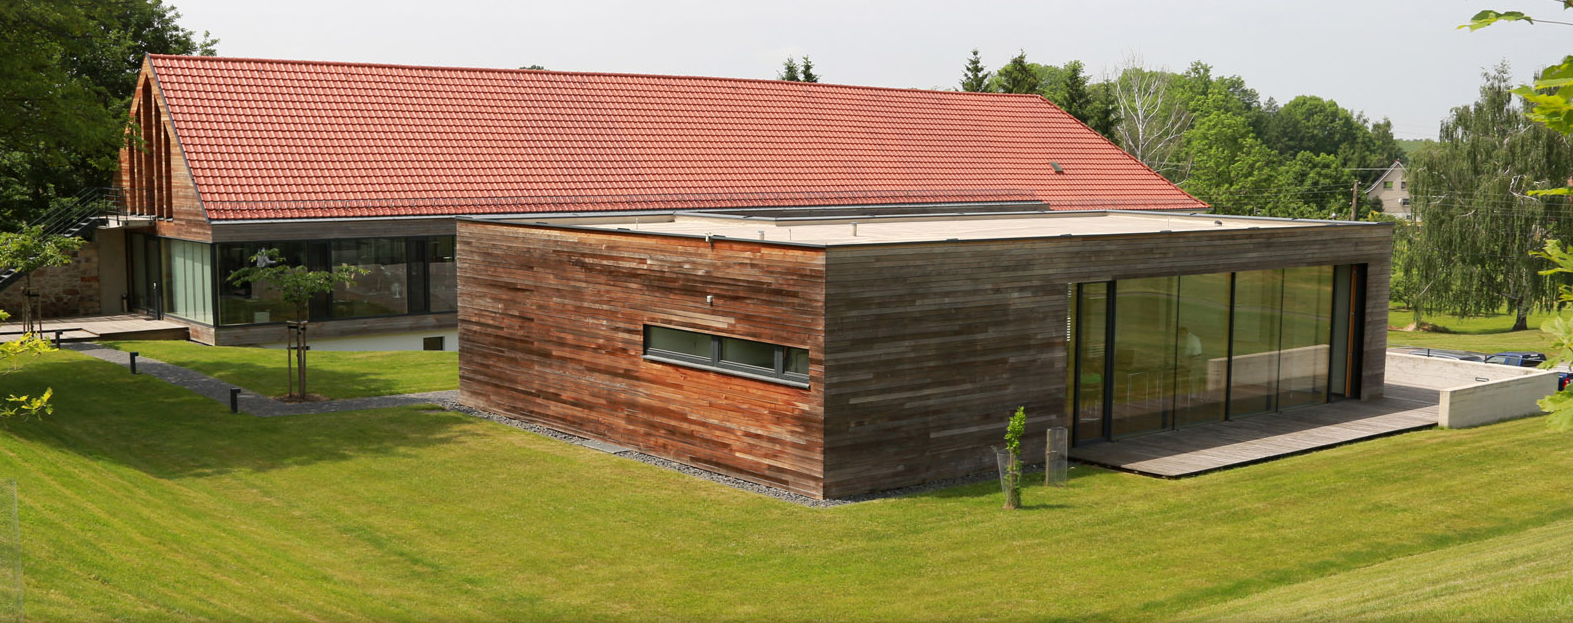
\includegraphics[scale=0.21]{Firma.png}
    %\caption{Image3.png}
\end{wrapfigure}
\underline{Unternehmen:}\\
Agri Con GmbH\\\url{http://agricon.de}\\
% Datenerfassung über Sensoren und Probenahmegräte 
% Technik (Elekktronik) und Erfahrungen
% Einsatzplanung von Maschinen, Betriebsmitteln und Arbeitszeit
% EInklang von Ertrags- und Qualitätsziele mit den wachsenden Umweltanforderungen
% Sensoren, GPS, Terminal, Telemetrie, Datenmanegement, Grunddüngung
\vspace{\baselineskip}
\vspace{\baselineskip}
\textit{Precision Farming}
\end{frame}

\begin{frame}\frametitle{Einleitung}
%TODO Abbildung von Anje
\begin{figure}
\centering
% Graphic for TeX using PGF
% Title: C:\Masterthesis\masterthesis\Abbildungen\Ist-Stand.dia
% Creator: Dia v0.97.2
% CreationDate: Thu Jan 22 16:24:29 2015
% For: KJunghanns
% \usepackage{tikz}
% The following commands are not supported in PSTricks at present
% We define them conditionally, so when they are implemented,
% this pgf file will use them.
\ifx\du\undefined
  \newlength{\du}
\fi
\setlength{\du}{15\unitlength}
\begin{tikzpicture}
\pgftransformxscale{1.000000}
\pgftransformyscale{-1.000000}
\definecolor{dialinecolor}{rgb}{0.000000, 0.000000, 0.000000}
\pgfsetstrokecolor{dialinecolor}
\definecolor{dialinecolor}{rgb}{1.000000, 1.000000, 1.000000}
\pgfsetfillcolor{dialinecolor}
\pgfsetlinewidth{0.080000\du}
\pgfsetdash{}{0pt}
\pgfsetdash{}{0pt}
\pgfsetbuttcap
\pgfsetmiterjoin
\pgfsetlinewidth{0.080000\du}
\pgfsetbuttcap
\pgfsetmiterjoin
\pgfsetdash{}{0pt}
\definecolor{dialinecolor}{rgb}{1.000000, 1.000000, 1.000000}
\pgfsetfillcolor{dialinecolor}
\pgfpathmoveto{\pgfpoint{18.749943\du}{9.336199\du}}
\pgfpathcurveto{\pgfpoint{17.508208\du}{9.323238\du}}{\pgfpoint{15.100000\du}{9.595408\du}}{\pgfpoint{15.438655\du}{10.178627\du}}
\pgfpathcurveto{\pgfpoint{15.777306\du}{10.761847\du}}{\pgfpoint{17.395323\du}{10.891446\du}}{\pgfpoint{18.072633\du}{10.722966\du}}
\pgfpathcurveto{\pgfpoint{18.749943\du}{10.554480\du}}{\pgfpoint{17.019040\du}{11.539468\du}}{\pgfpoint{20.330332\du}{11.798677\du}}
\pgfpathcurveto{\pgfpoint{23.641594\du}{12.057885\du}}{\pgfpoint{25.334868\du}{11.643151\du}}{\pgfpoint{24.845700\du}{11.345061\du}}
\pgfpathcurveto{\pgfpoint{24.356532\du}{11.046971\du}}{\pgfpoint{27.743080\du}{12.044925\du}}{\pgfpoint{29.323469\du}{11.474666\du}}
\pgfpathcurveto{\pgfpoint{30.903858\du}{10.904406\du}}{\pgfpoint{27.705452\du}{10.360073\du}}{\pgfpoint{28.382761\du}{10.437836\du}}
\pgfpathcurveto{\pgfpoint{29.060071\du}{10.515599\du}}{\pgfpoint{31.129628\du}{10.411915\du}}{\pgfpoint{30.452319\du}{9.439882\du}}
\pgfpathcurveto{\pgfpoint{29.775009\du}{8.467850\du}}{\pgfpoint{23.679222\du}{9.219555\du}}{\pgfpoint{24.356532\du}{9.076990\du}}
\pgfpathcurveto{\pgfpoint{25.033841\du}{8.934425\du}}{\pgfpoint{23.340567\du}{8.221600\du}}{\pgfpoint{21.233412\du}{8.364165\du}}
\pgfpathcurveto{\pgfpoint{19.126226\du}{8.506731\du}}{\pgfpoint{18.976766\du}{8.765434\du}}{\pgfpoint{18.750996\du}{9.335693\du}}
\pgfpathlineto{\pgfpoint{18.749943\du}{9.336199\du}}
\pgfusepath{fill}
\definecolor{dialinecolor}{rgb}{0.000000, 0.000000, 0.000000}
\pgfsetstrokecolor{dialinecolor}
\pgfpathmoveto{\pgfpoint{18.749943\du}{9.336199\du}}
\pgfpathcurveto{\pgfpoint{17.508208\du}{9.323238\du}}{\pgfpoint{15.100000\du}{9.595408\du}}{\pgfpoint{15.438655\du}{10.178627\du}}
\pgfpathcurveto{\pgfpoint{15.777306\du}{10.761847\du}}{\pgfpoint{17.395323\du}{10.891446\du}}{\pgfpoint{18.072633\du}{10.722966\du}}
\pgfpathcurveto{\pgfpoint{18.749943\du}{10.554480\du}}{\pgfpoint{17.019040\du}{11.539468\du}}{\pgfpoint{20.330332\du}{11.798677\du}}
\pgfpathcurveto{\pgfpoint{23.641594\du}{12.057885\du}}{\pgfpoint{25.334868\du}{11.643151\du}}{\pgfpoint{24.845700\du}{11.345061\du}}
\pgfpathcurveto{\pgfpoint{24.356532\du}{11.046971\du}}{\pgfpoint{27.743080\du}{12.044925\du}}{\pgfpoint{29.323469\du}{11.474666\du}}
\pgfpathcurveto{\pgfpoint{30.903858\du}{10.904406\du}}{\pgfpoint{27.705452\du}{10.360073\du}}{\pgfpoint{28.382761\du}{10.437836\du}}
\pgfpathcurveto{\pgfpoint{29.060071\du}{10.515599\du}}{\pgfpoint{31.129628\du}{10.411915\du}}{\pgfpoint{30.452319\du}{9.439882\du}}
\pgfpathcurveto{\pgfpoint{29.775009\du}{8.467850\du}}{\pgfpoint{23.679222\du}{9.219555\du}}{\pgfpoint{24.356532\du}{9.076990\du}}
\pgfpathcurveto{\pgfpoint{25.033841\du}{8.934425\du}}{\pgfpoint{23.340567\du}{8.221600\du}}{\pgfpoint{21.233412\du}{8.364165\du}}
\pgfpathcurveto{\pgfpoint{19.126226\du}{8.506731\du}}{\pgfpoint{18.976766\du}{8.765434\du}}{\pgfpoint{18.750996\du}{9.335693\du}}
\pgfpathlineto{\pgfpoint{18.749943\du}{9.336199\du}}
\pgfusepath{stroke}
% setfont left to latex
\definecolor{dialinecolor}{rgb}{0.000000, 0.000000, 0.000000}
\pgfsetstrokecolor{dialinecolor}
\node at (23.544513\du,10.079368\du){Sensoren, externe Unternehmen,};
% setfont left to latex
\definecolor{dialinecolor}{rgb}{0.000000, 0.000000, 0.000000}
\pgfsetstrokecolor{dialinecolor}
\node at (23.544513\du,10.719368\du){Mitarbeiter};
\pgfsetlinewidth{0.080000\du}
\pgfsetdash{}{0pt}
\pgfsetdash{}{0pt}
\pgfsetbuttcap
\pgfsetmiterjoin
\pgfsetlinewidth{0.080000\du}
\pgfsetbuttcap
\pgfsetmiterjoin
\pgfsetdash{}{0pt}
\definecolor{dialinecolor}{rgb}{1.000000, 1.000000, 1.000000}
\pgfsetfillcolor{dialinecolor}
\fill (22.430000\du,14.010000\du)--(22.430000\du,15.210000\du)--(23.790000\du,15.210000\du)--(23.790000\du,14.010000\du)--cycle;
\pgfsetbuttcap
\pgfsetmiterjoin
\pgfsetdash{}{0pt}
\definecolor{dialinecolor}{rgb}{1.000000, 1.000000, 1.000000}
\pgfsetfillcolor{dialinecolor}
\pgfpathellipse{\pgfpoint{23.110000\du}{15.210000\du}}{\pgfpoint{0.680000\du}{0\du}}{\pgfpoint{0\du}{0.200000\du}}
\pgfusepath{fill}
\pgfsetbuttcap
\pgfsetmiterjoin
\pgfsetdash{}{0pt}
\definecolor{dialinecolor}{rgb}{1.000000, 1.000000, 1.000000}
\pgfsetfillcolor{dialinecolor}
\pgfpathellipse{\pgfpoint{23.110000\du}{14.010000\du}}{\pgfpoint{0.680000\du}{0\du}}{\pgfpoint{0\du}{0.200000\du}}
\pgfusepath{fill}
\definecolor{dialinecolor}{rgb}{0.000000, 0.000000, 0.000000}
\pgfsetstrokecolor{dialinecolor}
\pgfpathellipse{\pgfpoint{23.110000\du}{14.010000\du}}{\pgfpoint{0.680000\du}{0\du}}{\pgfpoint{0\du}{0.200000\du}}
\pgfusepath{stroke}
\pgfsetbuttcap
\pgfsetmiterjoin
\pgfsetdash{}{0pt}
\definecolor{dialinecolor}{rgb}{0.000000, 0.000000, 0.000000}
\pgfsetstrokecolor{dialinecolor}
\pgfpathmoveto{\pgfpoint{23.790000\du}{14.010000\du}}
\pgfpathlineto{\pgfpoint{23.790000\du}{15.210000\du}}
\pgfpathcurveto{\pgfpoint{23.790000\du}{15.320457\du}}{\pgfpoint{23.485554\du}{15.410000\du}}{\pgfpoint{23.110000\du}{15.410000\du}}
\pgfpathcurveto{\pgfpoint{22.734446\du}{15.410000\du}}{\pgfpoint{22.430000\du}{15.320457\du}}{\pgfpoint{22.430000\du}{15.210000\du}}
\pgfpathlineto{\pgfpoint{22.430000\du}{14.010000\du}}
\pgfusepath{stroke}
% setfont left to latex
\definecolor{dialinecolor}{rgb}{0.000000, 0.000000, 0.000000}
\pgfsetstrokecolor{dialinecolor}
\node at (23.110000\du,15.922000\du){PostgreSQL};
\pgfsetlinewidth{0.080000\du}
\pgfsetdash{}{0pt}
\pgfsetdash{}{0pt}
\pgfsetbuttcap
\pgfsetmiterjoin
\pgfsetlinewidth{0.040000\du}
\pgfsetbuttcap
\pgfsetmiterjoin
\pgfsetdash{}{0pt}
\definecolor{dialinecolor}{rgb}{0.701961, 0.701961, 0.701961}
\pgfsetfillcolor{dialinecolor}
\fill (22.416500\du,18.250000\du)--(22.416500\du,19.470339\du)--(24.043619\du,19.470339\du)--(24.043619\du,18.250000\du)--cycle;
\definecolor{dialinecolor}{rgb}{0.000000, 0.000000, 0.000000}
\pgfsetstrokecolor{dialinecolor}
\draw (22.416500\du,18.250000\du)--(22.416500\du,19.470339\du)--(24.043619\du,19.470339\du)--(24.043619\du,18.250000\du)--cycle;
\pgfsetlinewidth{0.080000\du}
\pgfsetbuttcap
\pgfsetmiterjoin
\pgfsetdash{}{0pt}
\definecolor{dialinecolor}{rgb}{0.000000, 0.000000, 0.000000}
\pgfsetfillcolor{dialinecolor}
\fill (22.592771\du,18.426271\du)--(22.592771\du,19.266949\du)--(23.867347\du,19.266949\du)--(23.867347\du,18.426271\du)--cycle;
\pgfsetlinewidth{0.040000\du}
\pgfsetbuttcap
\pgfsetmiterjoin
\pgfsetdash{}{0pt}
\definecolor{dialinecolor}{rgb}{0.701961, 0.701961, 0.701961}
\pgfsetfillcolor{dialinecolor}
\fill (22.636839\du,19.470339\du)--(23.474127\du,19.470339\du)--(23.474127\du,19.660169\du)--(22.680907\du,19.660169\du)--cycle;
\definecolor{dialinecolor}{rgb}{0.000000, 0.000000, 0.000000}
\pgfsetstrokecolor{dialinecolor}
\draw (22.636839\du,19.470339\du)--(23.474127\du,19.470339\du)--(23.474127\du,19.660169\du)--(22.680907\du,19.660169\du)--cycle;
\pgfsetbuttcap
\pgfsetmiterjoin
\pgfsetdash{}{0pt}
\definecolor{dialinecolor}{rgb}{0.701961, 0.701961, 0.701961}
\pgfsetfillcolor{dialinecolor}
\fill (23.474127\du,19.470339\du)--(23.823280\du,19.470339\du)--(23.779212\du,19.660169\du)--(23.474127\du,19.660169\du)--cycle;
\definecolor{dialinecolor}{rgb}{0.000000, 0.000000, 0.000000}
\pgfsetstrokecolor{dialinecolor}
\draw (23.474127\du,19.470339\du)--(23.823280\du,19.470339\du)--(23.779212\du,19.660169\du)--(23.474127\du,19.660169\du)--cycle;
\pgfsetlinewidth{0.020000\du}
\pgfsetbuttcap
\pgfsetmiterjoin
\pgfsetdash{}{0pt}
\definecolor{dialinecolor}{rgb}{1.000000, 1.000000, 1.000000}
\pgfsetfillcolor{dialinecolor}
\fill (23.531076\du,19.527288\du)--(23.531076\du,19.603220\du)--(23.607008\du,19.603220\du)--(23.607008\du,19.527288\du)--cycle;
\definecolor{dialinecolor}{rgb}{0.000000, 0.000000, 0.000000}
\pgfsetstrokecolor{dialinecolor}
\draw (23.531076\du,19.527288\du)--(23.531076\du,19.603220\du)--(23.607008\du,19.603220\du)--(23.607008\du,19.527288\du)--cycle;
\pgfsetlinewidth{0.040000\du}
\pgfsetbuttcap
\pgfsetmiterjoin
\pgfsetdash{}{0pt}
\definecolor{dialinecolor}{rgb}{0.701961, 0.701961, 0.701961}
\pgfsetfillcolor{dialinecolor}
\fill (23.067347\du,19.660169\du)--(23.392771\du,19.660169\du)--(23.392771\du,19.755085\du)--(23.555483\du,19.755085\du)--(23.555483\du,19.850000\du)--(22.904636\du,19.850000\du)--(22.904636\du,19.755085\du)--(23.067347\du,19.755085\du)--cycle;
\definecolor{dialinecolor}{rgb}{0.000000, 0.000000, 0.000000}
\pgfsetstrokecolor{dialinecolor}
\draw (23.067347\du,19.660169\du)--(23.392771\du,19.660169\du)--(23.392771\du,19.755085\du)--(23.555483\du,19.755085\du)--(23.555483\du,19.850000\du)--(22.904636\du,19.850000\du)--(22.904636\du,19.755085\du)--(23.067347\du,19.755085\du)--cycle;
% setfont left to latex
\definecolor{dialinecolor}{rgb}{0.000000, 0.000000, 0.000000}
\pgfsetstrokecolor{dialinecolor}
\node at (23.230059\du,20.416237\du){Agriport};
\pgfsetlinewidth{0.080000\du}
\pgfsetdash{}{0pt}
\pgfsetdash{}{0pt}
\pgfsetbuttcap
\pgfsetmiterjoin
\pgfsetlinewidth{0.080000\du}
\pgfsetbuttcap
\pgfsetmiterjoin
\pgfsetdash{}{0pt}
\definecolor{dialinecolor}{rgb}{0.850980, 0.850980, 0.803922}
\pgfsetfillcolor{dialinecolor}
\fill (16.670000\du,12.730000\du)--(16.670000\du,13.580000\du)--(17.690000\du,13.580000\du)--(17.690000\du,12.730000\du)--cycle;
\definecolor{dialinecolor}{rgb}{0.000000, 0.000000, 0.000000}
\pgfsetstrokecolor{dialinecolor}
\draw (16.670000\du,12.730000\du)--(16.670000\du,13.580000\du)--(17.690000\du,13.580000\du)--(17.690000\du,12.730000\du)--cycle;
\pgfsetlinewidth{0.008000\du}
\pgfsetbuttcap
\pgfsetmiterjoin
\pgfsetdash{}{0pt}
\definecolor{dialinecolor}{rgb}{0.000000, 0.000000, 0.000000}
\pgfsetstrokecolor{dialinecolor}
\draw (16.670000\du,12.730000\du)--(16.670000\du,13.580000\du)--(17.690000\du,13.580000\du)--(17.690000\du,12.730000\du)--cycle;
\pgfsetlinewidth{0.080000\du}
\pgfsetbuttcap
\pgfsetmiterjoin
\pgfsetdash{}{0pt}
\definecolor{dialinecolor}{rgb}{0.631373, 0.631373, 0.631373}
\pgfsetfillcolor{dialinecolor}
\fill (16.726667\du,12.786667\du)--(16.726667\du,13.466667\du)--(17.633333\du,13.466667\du)--(17.633333\du,12.786667\du)--cycle;
\definecolor{dialinecolor}{rgb}{0.000000, 0.000000, 0.000000}
\pgfsetstrokecolor{dialinecolor}
\draw (16.726667\du,12.786667\du)--(16.726667\du,13.466667\du)--(17.633333\du,13.466667\du)--(17.633333\du,12.786667\du)--cycle;
\pgfsetlinewidth{0.008000\du}
\pgfsetbuttcap
\pgfsetmiterjoin
\pgfsetdash{}{0pt}
\definecolor{dialinecolor}{rgb}{0.000000, 0.000000, 0.000000}
\pgfsetstrokecolor{dialinecolor}
\draw (16.726667\du,12.786667\du)--(16.726667\du,13.466667\du)--(17.633333\du,13.466667\du)--(17.633333\du,12.786667\du)--cycle;
\pgfsetlinewidth{0.080000\du}
\pgfsetbuttcap
\pgfsetmiterjoin
\pgfsetdash{}{0pt}
\definecolor{dialinecolor}{rgb}{0.850980, 0.850980, 0.803922}
\pgfsetfillcolor{dialinecolor}
\fill (16.840000\du,13.580000\du)--(17.520000\du,13.580000\du)--(17.350000\du,13.636667\du)--(17.010000\du,13.636667\du)--cycle;
\definecolor{dialinecolor}{rgb}{0.000000, 0.000000, 0.000000}
\pgfsetstrokecolor{dialinecolor}
\draw (16.840000\du,13.580000\du)--(17.520000\du,13.580000\du)--(17.350000\du,13.636667\du)--(17.010000\du,13.636667\du)--cycle;
\pgfsetlinewidth{0.008000\du}
\pgfsetbuttcap
\pgfsetmiterjoin
\pgfsetdash{}{0pt}
\definecolor{dialinecolor}{rgb}{0.000000, 0.000000, 0.000000}
\pgfsetstrokecolor{dialinecolor}
\draw (16.840000\du,13.580000\du)--(17.520000\du,13.580000\du)--(17.350000\du,13.636667\du)--(17.010000\du,13.636667\du)--cycle;
\pgfsetlinewidth{0.080000\du}
\pgfsetbuttcap
\pgfsetmiterjoin
\pgfsetdash{}{0pt}
\definecolor{dialinecolor}{rgb}{0.850980, 0.850980, 0.803922}
\pgfsetfillcolor{dialinecolor}
\fill (17.010000\du,13.636667\du)--(17.010000\du,13.693333\du)--(17.350000\du,13.693333\du)--(17.350000\du,13.636667\du)--cycle;
\definecolor{dialinecolor}{rgb}{0.000000, 0.000000, 0.000000}
\pgfsetstrokecolor{dialinecolor}
\draw (17.010000\du,13.636667\du)--(17.010000\du,13.693333\du)--(17.350000\du,13.693333\du)--(17.350000\du,13.636667\du)--cycle;
\pgfsetlinewidth{0.008000\du}
\pgfsetbuttcap
\pgfsetmiterjoin
\pgfsetdash{}{0pt}
\definecolor{dialinecolor}{rgb}{0.000000, 0.000000, 0.000000}
\pgfsetstrokecolor{dialinecolor}
\draw (17.010000\du,13.636667\du)--(17.010000\du,13.693333\du)--(17.350000\du,13.693333\du)--(17.350000\du,13.636667\du)--cycle;
\pgfsetlinewidth{0.080000\du}
\pgfsetbuttcap
\pgfsetmiterjoin
\pgfsetdash{}{0pt}
\definecolor{dialinecolor}{rgb}{0.850980, 0.850980, 0.803922}
\pgfsetfillcolor{dialinecolor}
\fill (16.840000\du,13.693333\du)--(16.840000\du,13.750000\du)--(17.520000\du,13.750000\du)--(17.520000\du,13.693333\du)--cycle;
\definecolor{dialinecolor}{rgb}{0.000000, 0.000000, 0.000000}
\pgfsetstrokecolor{dialinecolor}
\draw (16.840000\du,13.693333\du)--(16.840000\du,13.750000\du)--(17.520000\du,13.750000\du)--(17.520000\du,13.693333\du)--cycle;
\pgfsetlinewidth{0.008000\du}
\pgfsetbuttcap
\pgfsetmiterjoin
\pgfsetdash{}{0pt}
\definecolor{dialinecolor}{rgb}{0.000000, 0.000000, 0.000000}
\pgfsetstrokecolor{dialinecolor}
\draw (16.840000\du,13.693333\du)--(16.840000\du,13.750000\du)--(17.520000\du,13.750000\du)--(17.520000\du,13.693333\du)--cycle;
\pgfsetlinewidth{0.080000\du}
\pgfsetdash{}{0pt}
\pgfsetdash{}{0pt}
\pgfsetbuttcap
\pgfsetmiterjoin
\pgfsetlinewidth{0.080000\du}
\pgfsetbuttcap
\pgfsetmiterjoin
\pgfsetdash{}{0pt}
\definecolor{dialinecolor}{rgb}{0.850980, 0.850980, 0.803922}
\pgfsetfillcolor{dialinecolor}
\fill (17.498500\du,14.398000\du)--(17.498500\du,15.248000\du)--(18.518500\du,15.248000\du)--(18.518500\du,14.398000\du)--cycle;
\definecolor{dialinecolor}{rgb}{0.000000, 0.000000, 0.000000}
\pgfsetstrokecolor{dialinecolor}
\draw (17.498500\du,14.398000\du)--(17.498500\du,15.248000\du)--(18.518500\du,15.248000\du)--(18.518500\du,14.398000\du)--cycle;
\pgfsetlinewidth{0.008000\du}
\pgfsetbuttcap
\pgfsetmiterjoin
\pgfsetdash{}{0pt}
\definecolor{dialinecolor}{rgb}{0.000000, 0.000000, 0.000000}
\pgfsetstrokecolor{dialinecolor}
\draw (17.498500\du,14.398000\du)--(17.498500\du,15.248000\du)--(18.518500\du,15.248000\du)--(18.518500\du,14.398000\du)--cycle;
\pgfsetlinewidth{0.080000\du}
\pgfsetbuttcap
\pgfsetmiterjoin
\pgfsetdash{}{0pt}
\definecolor{dialinecolor}{rgb}{0.631373, 0.631373, 0.631373}
\pgfsetfillcolor{dialinecolor}
\fill (17.555167\du,14.454667\du)--(17.555167\du,15.134667\du)--(18.461833\du,15.134667\du)--(18.461833\du,14.454667\du)--cycle;
\definecolor{dialinecolor}{rgb}{0.000000, 0.000000, 0.000000}
\pgfsetstrokecolor{dialinecolor}
\draw (17.555167\du,14.454667\du)--(17.555167\du,15.134667\du)--(18.461833\du,15.134667\du)--(18.461833\du,14.454667\du)--cycle;
\pgfsetlinewidth{0.008000\du}
\pgfsetbuttcap
\pgfsetmiterjoin
\pgfsetdash{}{0pt}
\definecolor{dialinecolor}{rgb}{0.000000, 0.000000, 0.000000}
\pgfsetstrokecolor{dialinecolor}
\draw (17.555167\du,14.454667\du)--(17.555167\du,15.134667\du)--(18.461833\du,15.134667\du)--(18.461833\du,14.454667\du)--cycle;
\pgfsetlinewidth{0.080000\du}
\pgfsetbuttcap
\pgfsetmiterjoin
\pgfsetdash{}{0pt}
\definecolor{dialinecolor}{rgb}{0.850980, 0.850980, 0.803922}
\pgfsetfillcolor{dialinecolor}
\fill (17.668500\du,15.248000\du)--(18.348500\du,15.248000\du)--(18.178500\du,15.304667\du)--(17.838500\du,15.304667\du)--cycle;
\definecolor{dialinecolor}{rgb}{0.000000, 0.000000, 0.000000}
\pgfsetstrokecolor{dialinecolor}
\draw (17.668500\du,15.248000\du)--(18.348500\du,15.248000\du)--(18.178500\du,15.304667\du)--(17.838500\du,15.304667\du)--cycle;
\pgfsetlinewidth{0.008000\du}
\pgfsetbuttcap
\pgfsetmiterjoin
\pgfsetdash{}{0pt}
\definecolor{dialinecolor}{rgb}{0.000000, 0.000000, 0.000000}
\pgfsetstrokecolor{dialinecolor}
\draw (17.668500\du,15.248000\du)--(18.348500\du,15.248000\du)--(18.178500\du,15.304667\du)--(17.838500\du,15.304667\du)--cycle;
\pgfsetlinewidth{0.080000\du}
\pgfsetbuttcap
\pgfsetmiterjoin
\pgfsetdash{}{0pt}
\definecolor{dialinecolor}{rgb}{0.850980, 0.850980, 0.803922}
\pgfsetfillcolor{dialinecolor}
\fill (17.838500\du,15.304667\du)--(17.838500\du,15.361333\du)--(18.178500\du,15.361333\du)--(18.178500\du,15.304667\du)--cycle;
\definecolor{dialinecolor}{rgb}{0.000000, 0.000000, 0.000000}
\pgfsetstrokecolor{dialinecolor}
\draw (17.838500\du,15.304667\du)--(17.838500\du,15.361333\du)--(18.178500\du,15.361333\du)--(18.178500\du,15.304667\du)--cycle;
\pgfsetlinewidth{0.008000\du}
\pgfsetbuttcap
\pgfsetmiterjoin
\pgfsetdash{}{0pt}
\definecolor{dialinecolor}{rgb}{0.000000, 0.000000, 0.000000}
\pgfsetstrokecolor{dialinecolor}
\draw (17.838500\du,15.304667\du)--(17.838500\du,15.361333\du)--(18.178500\du,15.361333\du)--(18.178500\du,15.304667\du)--cycle;
\pgfsetlinewidth{0.080000\du}
\pgfsetbuttcap
\pgfsetmiterjoin
\pgfsetdash{}{0pt}
\definecolor{dialinecolor}{rgb}{0.850980, 0.850980, 0.803922}
\pgfsetfillcolor{dialinecolor}
\fill (17.668500\du,15.361333\du)--(17.668500\du,15.418000\du)--(18.348500\du,15.418000\du)--(18.348500\du,15.361333\du)--cycle;
\definecolor{dialinecolor}{rgb}{0.000000, 0.000000, 0.000000}
\pgfsetstrokecolor{dialinecolor}
\draw (17.668500\du,15.361333\du)--(17.668500\du,15.418000\du)--(18.348500\du,15.418000\du)--(18.348500\du,15.361333\du)--cycle;
\pgfsetlinewidth{0.008000\du}
\pgfsetbuttcap
\pgfsetmiterjoin
\pgfsetdash{}{0pt}
\definecolor{dialinecolor}{rgb}{0.000000, 0.000000, 0.000000}
\pgfsetstrokecolor{dialinecolor}
\draw (17.668500\du,15.361333\du)--(17.668500\du,15.418000\du)--(18.348500\du,15.418000\du)--(18.348500\du,15.361333\du)--cycle;
\pgfsetlinewidth{0.080000\du}
\pgfsetdash{}{0pt}
\pgfsetdash{}{0pt}
\pgfsetbuttcap
\pgfsetmiterjoin
\pgfsetlinewidth{0.080000\du}
\pgfsetbuttcap
\pgfsetmiterjoin
\pgfsetdash{}{0pt}
\definecolor{dialinecolor}{rgb}{0.850980, 0.850980, 0.803922}
\pgfsetfillcolor{dialinecolor}
\fill (16.770500\du,15.946000\du)--(16.770500\du,16.796000\du)--(17.790500\du,16.796000\du)--(17.790500\du,15.946000\du)--cycle;
\definecolor{dialinecolor}{rgb}{0.000000, 0.000000, 0.000000}
\pgfsetstrokecolor{dialinecolor}
\draw (16.770500\du,15.946000\du)--(16.770500\du,16.796000\du)--(17.790500\du,16.796000\du)--(17.790500\du,15.946000\du)--cycle;
\pgfsetlinewidth{0.008000\du}
\pgfsetbuttcap
\pgfsetmiterjoin
\pgfsetdash{}{0pt}
\definecolor{dialinecolor}{rgb}{0.000000, 0.000000, 0.000000}
\pgfsetstrokecolor{dialinecolor}
\draw (16.770500\du,15.946000\du)--(16.770500\du,16.796000\du)--(17.790500\du,16.796000\du)--(17.790500\du,15.946000\du)--cycle;
\pgfsetlinewidth{0.080000\du}
\pgfsetbuttcap
\pgfsetmiterjoin
\pgfsetdash{}{0pt}
\definecolor{dialinecolor}{rgb}{0.631373, 0.631373, 0.631373}
\pgfsetfillcolor{dialinecolor}
\fill (16.827167\du,16.002667\du)--(16.827167\du,16.682667\du)--(17.733833\du,16.682667\du)--(17.733833\du,16.002667\du)--cycle;
\definecolor{dialinecolor}{rgb}{0.000000, 0.000000, 0.000000}
\pgfsetstrokecolor{dialinecolor}
\draw (16.827167\du,16.002667\du)--(16.827167\du,16.682667\du)--(17.733833\du,16.682667\du)--(17.733833\du,16.002667\du)--cycle;
\pgfsetlinewidth{0.008000\du}
\pgfsetbuttcap
\pgfsetmiterjoin
\pgfsetdash{}{0pt}
\definecolor{dialinecolor}{rgb}{0.000000, 0.000000, 0.000000}
\pgfsetstrokecolor{dialinecolor}
\draw (16.827167\du,16.002667\du)--(16.827167\du,16.682667\du)--(17.733833\du,16.682667\du)--(17.733833\du,16.002667\du)--cycle;
\pgfsetlinewidth{0.080000\du}
\pgfsetbuttcap
\pgfsetmiterjoin
\pgfsetdash{}{0pt}
\definecolor{dialinecolor}{rgb}{0.850980, 0.850980, 0.803922}
\pgfsetfillcolor{dialinecolor}
\fill (16.940500\du,16.796000\du)--(17.620500\du,16.796000\du)--(17.450500\du,16.852667\du)--(17.110500\du,16.852667\du)--cycle;
\definecolor{dialinecolor}{rgb}{0.000000, 0.000000, 0.000000}
\pgfsetstrokecolor{dialinecolor}
\draw (16.940500\du,16.796000\du)--(17.620500\du,16.796000\du)--(17.450500\du,16.852667\du)--(17.110500\du,16.852667\du)--cycle;
\pgfsetlinewidth{0.008000\du}
\pgfsetbuttcap
\pgfsetmiterjoin
\pgfsetdash{}{0pt}
\definecolor{dialinecolor}{rgb}{0.000000, 0.000000, 0.000000}
\pgfsetstrokecolor{dialinecolor}
\draw (16.940500\du,16.796000\du)--(17.620500\du,16.796000\du)--(17.450500\du,16.852667\du)--(17.110500\du,16.852667\du)--cycle;
\pgfsetlinewidth{0.080000\du}
\pgfsetbuttcap
\pgfsetmiterjoin
\pgfsetdash{}{0pt}
\definecolor{dialinecolor}{rgb}{0.850980, 0.850980, 0.803922}
\pgfsetfillcolor{dialinecolor}
\fill (17.110500\du,16.852667\du)--(17.110500\du,16.909333\du)--(17.450500\du,16.909333\du)--(17.450500\du,16.852667\du)--cycle;
\definecolor{dialinecolor}{rgb}{0.000000, 0.000000, 0.000000}
\pgfsetstrokecolor{dialinecolor}
\draw (17.110500\du,16.852667\du)--(17.110500\du,16.909333\du)--(17.450500\du,16.909333\du)--(17.450500\du,16.852667\du)--cycle;
\pgfsetlinewidth{0.008000\du}
\pgfsetbuttcap
\pgfsetmiterjoin
\pgfsetdash{}{0pt}
\definecolor{dialinecolor}{rgb}{0.000000, 0.000000, 0.000000}
\pgfsetstrokecolor{dialinecolor}
\draw (17.110500\du,16.852667\du)--(17.110500\du,16.909333\du)--(17.450500\du,16.909333\du)--(17.450500\du,16.852667\du)--cycle;
\pgfsetlinewidth{0.080000\du}
\pgfsetbuttcap
\pgfsetmiterjoin
\pgfsetdash{}{0pt}
\definecolor{dialinecolor}{rgb}{0.850980, 0.850980, 0.803922}
\pgfsetfillcolor{dialinecolor}
\fill (16.940500\du,16.909333\du)--(16.940500\du,16.966000\du)--(17.620500\du,16.966000\du)--(17.620500\du,16.909333\du)--cycle;
\definecolor{dialinecolor}{rgb}{0.000000, 0.000000, 0.000000}
\pgfsetstrokecolor{dialinecolor}
\draw (16.940500\du,16.909333\du)--(16.940500\du,16.966000\du)--(17.620500\du,16.966000\du)--(17.620500\du,16.909333\du)--cycle;
\pgfsetlinewidth{0.008000\du}
\pgfsetbuttcap
\pgfsetmiterjoin
\pgfsetdash{}{0pt}
\definecolor{dialinecolor}{rgb}{0.000000, 0.000000, 0.000000}
\pgfsetstrokecolor{dialinecolor}
\draw (16.940500\du,16.909333\du)--(16.940500\du,16.966000\du)--(17.620500\du,16.966000\du)--(17.620500\du,16.909333\du)--cycle;
% setfont left to latex
\definecolor{dialinecolor}{rgb}{0.000000, 0.000000, 0.000000}
\pgfsetstrokecolor{dialinecolor}
\node[anchor=west] at (15.590000\du,17.730000\du){Agri Con Intern};
\pgfsetlinewidth{0.080000\du}
\pgfsetdash{}{0pt}
\pgfsetdash{}{0pt}
\pgfsetbuttcap
{
\definecolor{dialinecolor}{rgb}{0.000000, 0.000000, 0.000000}
\pgfsetfillcolor{dialinecolor}
% was here!!!
\pgfsetarrowsend{stealth}
\definecolor{dialinecolor}{rgb}{0.000000, 0.000000, 0.000000}
\pgfsetstrokecolor{dialinecolor}
\draw (23.167337\du,11.886149\du)--(23.210796\du,13.775218\du);
}
\pgfsetlinewidth{0.080000\du}
\pgfsetdash{}{0pt}
\pgfsetdash{}{0pt}
\pgfsetbuttcap
{
\definecolor{dialinecolor}{rgb}{0.000000, 0.000000, 0.000000}
\pgfsetfillcolor{dialinecolor}
% was here!!!
\pgfsetarrowsstart{stealth}
\pgfsetarrowsend{latex}
\definecolor{dialinecolor}{rgb}{0.000000, 0.000000, 0.000000}
\pgfsetstrokecolor{dialinecolor}
\draw (23.238032\du,16.373080\du)--(23.232496\du,18.231762\du);
}
\pgfsetlinewidth{0.080000\du}
\pgfsetdash{}{0pt}
\pgfsetdash{}{0pt}
\pgfsetbuttcap
{
\definecolor{dialinecolor}{rgb}{0.000000, 0.000000, 0.000000}
\pgfsetfillcolor{dialinecolor}
% was here!!!
\pgfsetarrowsstart{latex}
\pgfsetarrowsend{latex}
\definecolor{dialinecolor}{rgb}{0.000000, 0.000000, 0.000000}
\pgfsetstrokecolor{dialinecolor}
\draw (22.391973\du,14.610000\du)--(18.950000\du,14.610000\du);
}
\pgfsetlinewidth{0.080000\du}
\pgfsetdash{}{0pt}
\pgfsetdash{}{0pt}
\pgfsetbuttcap
{
\definecolor{dialinecolor}{rgb}{0.000000, 0.000000, 0.000000}
\pgfsetfillcolor{dialinecolor}
% was here!!!
\pgfsetarrowsend{latex}
\definecolor{dialinecolor}{rgb}{0.000000, 0.000000, 0.000000}
\pgfsetstrokecolor{dialinecolor}
\pgfpathmoveto{\pgfpoint{23.821525\du}{16.535113\du}}
\pgfpatharc{131}{-128}{1.640858\du and 1.640858\du}
\pgfusepath{stroke}
}
% setfont left to latex
\definecolor{dialinecolor}{rgb}{0.000000, 0.000000, 0.000000}
\pgfsetstrokecolor{dialinecolor}
\node[anchor=west] at (26.722640\du,14.883849\du){Batch};
% setfont left to latex
\definecolor{dialinecolor}{rgb}{0.000000, 0.000000, 0.000000}
\pgfsetstrokecolor{dialinecolor}
\node[anchor=west] at (26.722640\du,15.523849\du){Vorgänge};
\end{tikzpicture}

\caption{Aktueller Stand bei Agri Con}
\end{figure}
\end{frame}

\begin{frame}\frametitle{Einleitung}
%TODO Abbildung von Anje
\begin{figure}[h!]
\centering
\resizebox{.92\linewidth}{!}{% Graphic for TeX using PGF
% Title: C:\Masterthesis\masterthesis\Abbildungen\Wunsch-Stand.dia
% Creator: Dia v0.97.2
% CreationDate: Thu Jan 22 16:40:13 2015
% For: KJunghanns
% \usepackage{tikz}
% The following commands are not supported in PSTricks at present
% We define them conditionally, so when they are implemented,
% this pgf file will use them.
\ifx\du\undefined
  \newlength{\du}
\fi
\setlength{\du}{15\unitlength}
\begin{tikzpicture}
\pgftransformxscale{1.000000}
\pgftransformyscale{-1.000000}
\definecolor{dialinecolor}{rgb}{0.000000, 0.000000, 0.000000}
\pgfsetstrokecolor{dialinecolor}
\definecolor{dialinecolor}{rgb}{1.000000, 1.000000, 1.000000}
\pgfsetfillcolor{dialinecolor}
\pgfsetlinewidth{0.100000\du}
\pgfsetdash{}{0pt}
\pgfsetdash{}{0pt}
\pgfsetbuttcap
\pgfsetmiterjoin
\pgfsetlinewidth{0.100000\du}
\pgfsetbuttcap
\pgfsetmiterjoin
\pgfsetdash{}{0pt}
\definecolor{dialinecolor}{rgb}{1.000000, 1.000000, 1.000000}
\pgfsetfillcolor{dialinecolor}
\pgfpathmoveto{\pgfpoint{16.667981\du}{7.329099\du}}
\pgfpathcurveto{\pgfpoint{15.122429\du}{7.316138\du}}{\pgfpoint{12.125000\du}{7.588308\du}}{\pgfpoint{12.546514\du}{8.171527\du}}
\pgfpathcurveto{\pgfpoint{12.968024\du}{8.754747\du}}{\pgfpoint{14.981924\du}{8.884346\du}}{\pgfpoint{15.824953\du}{8.715866\du}}
\pgfpathcurveto{\pgfpoint{16.667981\du}{8.547380\du}}{\pgfpoint{14.513575\du}{9.532368\du}}{\pgfpoint{18.635047\du}{9.791577\du}}
\pgfpathcurveto{\pgfpoint{22.756481\du}{10.050785\du}}{\pgfpoint{24.864051\du}{9.636051\du}}{\pgfpoint{24.255197\du}{9.337961\du}}
\pgfpathcurveto{\pgfpoint{23.646344\du}{9.039871\du}}{\pgfpoint{27.861485\du}{10.037825\du}}{\pgfpoint{29.828551\du}{9.467566\du}}
\pgfpathcurveto{\pgfpoint{31.795617\du}{8.897306\du}}{\pgfpoint{27.814650\du}{8.352973\du}}{\pgfpoint{28.657678\du}{8.430736\du}}
\pgfpathcurveto{\pgfpoint{29.500706\du}{8.508499\du}}{\pgfpoint{32.076626\du}{8.404815\du}}{\pgfpoint{31.233598\du}{7.432782\du}}
\pgfpathcurveto{\pgfpoint{30.390569\du}{6.460750\du}}{\pgfpoint{22.803315\du}{7.212455\du}}{\pgfpoint{23.646344\du}{7.069890\du}}
\pgfpathcurveto{\pgfpoint{24.489372\du}{6.927325\du}}{\pgfpoint{22.381801\du}{6.214500\du}}{\pgfpoint{19.759084\du}{6.357065\du}}
\pgfpathcurveto{\pgfpoint{17.136330\du}{6.499631\du}}{\pgfpoint{16.950302\du}{6.758334\du}}{\pgfpoint{16.669292\du}{7.328593\du}}
\pgfpathlineto{\pgfpoint{16.667981\du}{7.329099\du}}
\pgfusepath{fill}
\definecolor{dialinecolor}{rgb}{0.000000, 0.000000, 0.000000}
\pgfsetstrokecolor{dialinecolor}
\pgfpathmoveto{\pgfpoint{16.667981\du}{7.329099\du}}
\pgfpathcurveto{\pgfpoint{15.122429\du}{7.316138\du}}{\pgfpoint{12.125000\du}{7.588308\du}}{\pgfpoint{12.546514\du}{8.171527\du}}
\pgfpathcurveto{\pgfpoint{12.968024\du}{8.754747\du}}{\pgfpoint{14.981924\du}{8.884346\du}}{\pgfpoint{15.824953\du}{8.715866\du}}
\pgfpathcurveto{\pgfpoint{16.667981\du}{8.547380\du}}{\pgfpoint{14.513575\du}{9.532368\du}}{\pgfpoint{18.635047\du}{9.791577\du}}
\pgfpathcurveto{\pgfpoint{22.756481\du}{10.050785\du}}{\pgfpoint{24.864051\du}{9.636051\du}}{\pgfpoint{24.255197\du}{9.337961\du}}
\pgfpathcurveto{\pgfpoint{23.646344\du}{9.039871\du}}{\pgfpoint{27.861485\du}{10.037825\du}}{\pgfpoint{29.828551\du}{9.467566\du}}
\pgfpathcurveto{\pgfpoint{31.795617\du}{8.897306\du}}{\pgfpoint{27.814650\du}{8.352973\du}}{\pgfpoint{28.657678\du}{8.430736\du}}
\pgfpathcurveto{\pgfpoint{29.500706\du}{8.508499\du}}{\pgfpoint{32.076626\du}{8.404815\du}}{\pgfpoint{31.233598\du}{7.432782\du}}
\pgfpathcurveto{\pgfpoint{30.390569\du}{6.460750\du}}{\pgfpoint{22.803315\du}{7.212455\du}}{\pgfpoint{23.646344\du}{7.069890\du}}
\pgfpathcurveto{\pgfpoint{24.489372\du}{6.927325\du}}{\pgfpoint{22.381801\du}{6.214500\du}}{\pgfpoint{19.759084\du}{6.357065\du}}
\pgfpathcurveto{\pgfpoint{17.136330\du}{6.499631\du}}{\pgfpoint{16.950302\du}{6.758334\du}}{\pgfpoint{16.669292\du}{7.328593\du}}
\pgfpathlineto{\pgfpoint{16.667981\du}{7.329099\du}}
\pgfusepath{stroke}
% setfont left to latex
\definecolor{dialinecolor}{rgb}{0.000000, 0.000000, 0.000000}
\pgfsetstrokecolor{dialinecolor}
\node at (22.635646\du,8.040268\du){Sensoren, externe Unternehmen,};
% setfont left to latex
\definecolor{dialinecolor}{rgb}{0.000000, 0.000000, 0.000000}
\pgfsetstrokecolor{dialinecolor}
\node at (22.635646\du,8.840268\du){Mitarbeiter};
\pgfsetlinewidth{0.100000\du}
\pgfsetdash{}{0pt}
\pgfsetdash{}{0pt}
\pgfsetbuttcap
\pgfsetmiterjoin
\pgfsetlinewidth{0.100000\du}
\pgfsetbuttcap
\pgfsetmiterjoin
\pgfsetdash{}{0pt}
\definecolor{dialinecolor}{rgb}{1.000000, 1.000000, 1.000000}
\pgfsetfillcolor{dialinecolor}
\fill (21.100000\du,13.450000\du)--(21.100000\du,14.950000\du)--(22.800000\du,14.950000\du)--(22.800000\du,13.450000\du)--cycle;
\pgfsetbuttcap
\pgfsetmiterjoin
\pgfsetdash{}{0pt}
\definecolor{dialinecolor}{rgb}{1.000000, 1.000000, 1.000000}
\pgfsetfillcolor{dialinecolor}
\pgfpathellipse{\pgfpoint{21.950000\du}{14.950000\du}}{\pgfpoint{0.850000\du}{0\du}}{\pgfpoint{0\du}{0.250000\du}}
\pgfusepath{fill}
\pgfsetbuttcap
\pgfsetmiterjoin
\pgfsetdash{}{0pt}
\definecolor{dialinecolor}{rgb}{1.000000, 1.000000, 1.000000}
\pgfsetfillcolor{dialinecolor}
\pgfpathellipse{\pgfpoint{21.950000\du}{13.450000\du}}{\pgfpoint{0.850000\du}{0\du}}{\pgfpoint{0\du}{0.250000\du}}
\pgfusepath{fill}
\definecolor{dialinecolor}{rgb}{0.000000, 0.000000, 0.000000}
\pgfsetstrokecolor{dialinecolor}
\pgfpathellipse{\pgfpoint{21.950000\du}{13.450000\du}}{\pgfpoint{0.850000\du}{0\du}}{\pgfpoint{0\du}{0.250000\du}}
\pgfusepath{stroke}
\pgfsetbuttcap
\pgfsetmiterjoin
\pgfsetdash{}{0pt}
\definecolor{dialinecolor}{rgb}{0.000000, 0.000000, 0.000000}
\pgfsetstrokecolor{dialinecolor}
\pgfpathmoveto{\pgfpoint{22.800000\du}{13.450000\du}}
\pgfpathlineto{\pgfpoint{22.800000\du}{14.950000\du}}
\pgfpathcurveto{\pgfpoint{22.800000\du}{15.088071\du}}{\pgfpoint{22.419442\du}{15.200000\du}}{\pgfpoint{21.950000\du}{15.200000\du}}
\pgfpathcurveto{\pgfpoint{21.480558\du}{15.200000\du}}{\pgfpoint{21.100000\du}{15.088071\du}}{\pgfpoint{21.100000\du}{14.950000\du}}
\pgfpathlineto{\pgfpoint{21.100000\du}{13.450000\du}}
\pgfusepath{stroke}
% setfont left to latex
\definecolor{dialinecolor}{rgb}{0.000000, 0.000000, 0.000000}
\pgfsetstrokecolor{dialinecolor}
\node at (21.950000\du,15.840000\du){PostgreSQL};
\pgfsetlinewidth{0.100000\du}
\pgfsetdash{}{0pt}
\pgfsetdash{}{0pt}
\pgfsetbuttcap
\pgfsetmiterjoin
\pgfsetlinewidth{0.050000\du}
\pgfsetbuttcap
\pgfsetmiterjoin
\pgfsetdash{}{0pt}
\definecolor{dialinecolor}{rgb}{0.701961, 0.701961, 0.701961}
\pgfsetfillcolor{dialinecolor}
\fill (21.083100\du,18.750000\du)--(21.083100\du,20.275424\du)--(23.116998\du,20.275424\du)--(23.116998\du,18.750000\du)--cycle;
\definecolor{dialinecolor}{rgb}{0.000000, 0.000000, 0.000000}
\pgfsetstrokecolor{dialinecolor}
\draw (21.083100\du,18.750000\du)--(21.083100\du,20.275424\du)--(23.116998\du,20.275424\du)--(23.116998\du,18.750000\du)--cycle;
\pgfsetlinewidth{0.100000\du}
\pgfsetbuttcap
\pgfsetmiterjoin
\pgfsetdash{}{0pt}
\definecolor{dialinecolor}{rgb}{0.000000, 0.000000, 0.000000}
\pgfsetfillcolor{dialinecolor}
\fill (21.303439\du,18.970339\du)--(21.303439\du,20.021186\du)--(22.896659\du,20.021186\du)--(22.896659\du,18.970339\du)--cycle;
\pgfsetlinewidth{0.050000\du}
\pgfsetbuttcap
\pgfsetmiterjoin
\pgfsetdash{}{0pt}
\definecolor{dialinecolor}{rgb}{0.701961, 0.701961, 0.701961}
\pgfsetfillcolor{dialinecolor}
\fill (21.358524\du,20.275424\du)--(22.405134\du,20.275424\du)--(22.405134\du,20.512712\du)--(21.413608\du,20.512712\du)--cycle;
\definecolor{dialinecolor}{rgb}{0.000000, 0.000000, 0.000000}
\pgfsetstrokecolor{dialinecolor}
\draw (21.358524\du,20.275424\du)--(22.405134\du,20.275424\du)--(22.405134\du,20.512712\du)--(21.413608\du,20.512712\du)--cycle;
\pgfsetbuttcap
\pgfsetmiterjoin
\pgfsetdash{}{0pt}
\definecolor{dialinecolor}{rgb}{0.701961, 0.701961, 0.701961}
\pgfsetfillcolor{dialinecolor}
\fill (22.405134\du,20.275424\du)--(22.841575\du,20.275424\du)--(22.786490\du,20.512712\du)--(22.405134\du,20.512712\du)--cycle;
\definecolor{dialinecolor}{rgb}{0.000000, 0.000000, 0.000000}
\pgfsetstrokecolor{dialinecolor}
\draw (22.405134\du,20.275424\du)--(22.841575\du,20.275424\du)--(22.786490\du,20.512712\du)--(22.405134\du,20.512712\du)--cycle;
\pgfsetlinewidth{0.025000\du}
\pgfsetbuttcap
\pgfsetmiterjoin
\pgfsetdash{}{0pt}
\definecolor{dialinecolor}{rgb}{1.000000, 1.000000, 1.000000}
\pgfsetfillcolor{dialinecolor}
\fill (22.476320\du,20.346610\du)--(22.476320\du,20.441525\du)--(22.571236\du,20.441525\du)--(22.571236\du,20.346610\du)--cycle;
\definecolor{dialinecolor}{rgb}{0.000000, 0.000000, 0.000000}
\pgfsetstrokecolor{dialinecolor}
\draw (22.476320\du,20.346610\du)--(22.476320\du,20.441525\du)--(22.571236\du,20.441525\du)--(22.571236\du,20.346610\du)--cycle;
\pgfsetlinewidth{0.050000\du}
\pgfsetbuttcap
\pgfsetmiterjoin
\pgfsetdash{}{0pt}
\definecolor{dialinecolor}{rgb}{0.701961, 0.701961, 0.701961}
\pgfsetfillcolor{dialinecolor}
\fill (21.896659\du,20.512712\du)--(22.303439\du,20.512712\du)--(22.303439\du,20.631356\du)--(22.506829\du,20.631356\du)--(22.506829\du,20.750000\du)--(21.693269\du,20.750000\du)--(21.693269\du,20.631356\du)--(21.896659\du,20.631356\du)--cycle;
\definecolor{dialinecolor}{rgb}{0.000000, 0.000000, 0.000000}
\pgfsetstrokecolor{dialinecolor}
\draw (21.896659\du,20.512712\du)--(22.303439\du,20.512712\du)--(22.303439\du,20.631356\du)--(22.506829\du,20.631356\du)--(22.506829\du,20.750000\du)--(21.693269\du,20.750000\du)--(21.693269\du,20.631356\du)--(21.896659\du,20.631356\du)--cycle;
% setfont left to latex
\definecolor{dialinecolor}{rgb}{0.000000, 0.000000, 0.000000}
\pgfsetstrokecolor{dialinecolor}
\node at (22.100049\du,21.457797\du){Agriport};
\pgfsetlinewidth{0.100000\du}
\pgfsetdash{}{0pt}
\pgfsetdash{}{0pt}
\pgfsetbuttcap
\pgfsetmiterjoin
\pgfsetlinewidth{0.100000\du}
\pgfsetbuttcap
\pgfsetmiterjoin
\pgfsetdash{}{0pt}
\definecolor{dialinecolor}{rgb}{0.850980, 0.850980, 0.803922}
\pgfsetfillcolor{dialinecolor}
\fill (13.900000\du,11.850000\du)--(13.900000\du,12.912500\du)--(15.175000\du,12.912500\du)--(15.175000\du,11.850000\du)--cycle;
\definecolor{dialinecolor}{rgb}{0.000000, 0.000000, 0.000000}
\pgfsetstrokecolor{dialinecolor}
\draw (13.900000\du,11.850000\du)--(13.900000\du,12.912500\du)--(15.175000\du,12.912500\du)--(15.175000\du,11.850000\du)--cycle;
\pgfsetlinewidth{0.010000\du}
\pgfsetbuttcap
\pgfsetmiterjoin
\pgfsetdash{}{0pt}
\definecolor{dialinecolor}{rgb}{0.000000, 0.000000, 0.000000}
\pgfsetstrokecolor{dialinecolor}
\draw (13.900000\du,11.850000\du)--(13.900000\du,12.912500\du)--(15.175000\du,12.912500\du)--(15.175000\du,11.850000\du)--cycle;
\pgfsetlinewidth{0.100000\du}
\pgfsetbuttcap
\pgfsetmiterjoin
\pgfsetdash{}{0pt}
\definecolor{dialinecolor}{rgb}{0.631373, 0.631373, 0.631373}
\pgfsetfillcolor{dialinecolor}
\fill (13.970833\du,11.920833\du)--(13.970833\du,12.770833\du)--(15.104167\du,12.770833\du)--(15.104167\du,11.920833\du)--cycle;
\definecolor{dialinecolor}{rgb}{0.000000, 0.000000, 0.000000}
\pgfsetstrokecolor{dialinecolor}
\draw (13.970833\du,11.920833\du)--(13.970833\du,12.770833\du)--(15.104167\du,12.770833\du)--(15.104167\du,11.920833\du)--cycle;
\pgfsetlinewidth{0.010000\du}
\pgfsetbuttcap
\pgfsetmiterjoin
\pgfsetdash{}{0pt}
\definecolor{dialinecolor}{rgb}{0.000000, 0.000000, 0.000000}
\pgfsetstrokecolor{dialinecolor}
\draw (13.970833\du,11.920833\du)--(13.970833\du,12.770833\du)--(15.104167\du,12.770833\du)--(15.104167\du,11.920833\du)--cycle;
\pgfsetlinewidth{0.100000\du}
\pgfsetbuttcap
\pgfsetmiterjoin
\pgfsetdash{}{0pt}
\definecolor{dialinecolor}{rgb}{0.850980, 0.850980, 0.803922}
\pgfsetfillcolor{dialinecolor}
\fill (14.112500\du,12.912500\du)--(14.962500\du,12.912500\du)--(14.750000\du,12.983333\du)--(14.325000\du,12.983333\du)--cycle;
\definecolor{dialinecolor}{rgb}{0.000000, 0.000000, 0.000000}
\pgfsetstrokecolor{dialinecolor}
\draw (14.112500\du,12.912500\du)--(14.962500\du,12.912500\du)--(14.750000\du,12.983333\du)--(14.325000\du,12.983333\du)--cycle;
\pgfsetlinewidth{0.010000\du}
\pgfsetbuttcap
\pgfsetmiterjoin
\pgfsetdash{}{0pt}
\definecolor{dialinecolor}{rgb}{0.000000, 0.000000, 0.000000}
\pgfsetstrokecolor{dialinecolor}
\draw (14.112500\du,12.912500\du)--(14.962500\du,12.912500\du)--(14.750000\du,12.983333\du)--(14.325000\du,12.983333\du)--cycle;
\pgfsetlinewidth{0.100000\du}
\pgfsetbuttcap
\pgfsetmiterjoin
\pgfsetdash{}{0pt}
\definecolor{dialinecolor}{rgb}{0.850980, 0.850980, 0.803922}
\pgfsetfillcolor{dialinecolor}
\fill (14.325000\du,12.983333\du)--(14.325000\du,13.054167\du)--(14.750000\du,13.054167\du)--(14.750000\du,12.983333\du)--cycle;
\definecolor{dialinecolor}{rgb}{0.000000, 0.000000, 0.000000}
\pgfsetstrokecolor{dialinecolor}
\draw (14.325000\du,12.983333\du)--(14.325000\du,13.054167\du)--(14.750000\du,13.054167\du)--(14.750000\du,12.983333\du)--cycle;
\pgfsetlinewidth{0.010000\du}
\pgfsetbuttcap
\pgfsetmiterjoin
\pgfsetdash{}{0pt}
\definecolor{dialinecolor}{rgb}{0.000000, 0.000000, 0.000000}
\pgfsetstrokecolor{dialinecolor}
\draw (14.325000\du,12.983333\du)--(14.325000\du,13.054167\du)--(14.750000\du,13.054167\du)--(14.750000\du,12.983333\du)--cycle;
\pgfsetlinewidth{0.100000\du}
\pgfsetbuttcap
\pgfsetmiterjoin
\pgfsetdash{}{0pt}
\definecolor{dialinecolor}{rgb}{0.850980, 0.850980, 0.803922}
\pgfsetfillcolor{dialinecolor}
\fill (14.112500\du,13.054167\du)--(14.112500\du,13.125000\du)--(14.962500\du,13.125000\du)--(14.962500\du,13.054167\du)--cycle;
\definecolor{dialinecolor}{rgb}{0.000000, 0.000000, 0.000000}
\pgfsetstrokecolor{dialinecolor}
\draw (14.112500\du,13.054167\du)--(14.112500\du,13.125000\du)--(14.962500\du,13.125000\du)--(14.962500\du,13.054167\du)--cycle;
\pgfsetlinewidth{0.010000\du}
\pgfsetbuttcap
\pgfsetmiterjoin
\pgfsetdash{}{0pt}
\definecolor{dialinecolor}{rgb}{0.000000, 0.000000, 0.000000}
\pgfsetstrokecolor{dialinecolor}
\draw (14.112500\du,13.054167\du)--(14.112500\du,13.125000\du)--(14.962500\du,13.125000\du)--(14.962500\du,13.054167\du)--cycle;
\pgfsetlinewidth{0.100000\du}
\pgfsetdash{}{0pt}
\pgfsetdash{}{0pt}
\pgfsetbuttcap
\pgfsetmiterjoin
\pgfsetlinewidth{0.100000\du}
\pgfsetbuttcap
\pgfsetmiterjoin
\pgfsetdash{}{0pt}
\definecolor{dialinecolor}{rgb}{0.850980, 0.850980, 0.803922}
\pgfsetfillcolor{dialinecolor}
\fill (14.935600\du,13.935000\du)--(14.935600\du,14.997500\du)--(16.210600\du,14.997500\du)--(16.210600\du,13.935000\du)--cycle;
\definecolor{dialinecolor}{rgb}{0.000000, 0.000000, 0.000000}
\pgfsetstrokecolor{dialinecolor}
\draw (14.935600\du,13.935000\du)--(14.935600\du,14.997500\du)--(16.210600\du,14.997500\du)--(16.210600\du,13.935000\du)--cycle;
\pgfsetlinewidth{0.010000\du}
\pgfsetbuttcap
\pgfsetmiterjoin
\pgfsetdash{}{0pt}
\definecolor{dialinecolor}{rgb}{0.000000, 0.000000, 0.000000}
\pgfsetstrokecolor{dialinecolor}
\draw (14.935600\du,13.935000\du)--(14.935600\du,14.997500\du)--(16.210600\du,14.997500\du)--(16.210600\du,13.935000\du)--cycle;
\pgfsetlinewidth{0.100000\du}
\pgfsetbuttcap
\pgfsetmiterjoin
\pgfsetdash{}{0pt}
\definecolor{dialinecolor}{rgb}{0.631373, 0.631373, 0.631373}
\pgfsetfillcolor{dialinecolor}
\fill (15.006433\du,14.005833\du)--(15.006433\du,14.855833\du)--(16.139767\du,14.855833\du)--(16.139767\du,14.005833\du)--cycle;
\definecolor{dialinecolor}{rgb}{0.000000, 0.000000, 0.000000}
\pgfsetstrokecolor{dialinecolor}
\draw (15.006433\du,14.005833\du)--(15.006433\du,14.855833\du)--(16.139767\du,14.855833\du)--(16.139767\du,14.005833\du)--cycle;
\pgfsetlinewidth{0.010000\du}
\pgfsetbuttcap
\pgfsetmiterjoin
\pgfsetdash{}{0pt}
\definecolor{dialinecolor}{rgb}{0.000000, 0.000000, 0.000000}
\pgfsetstrokecolor{dialinecolor}
\draw (15.006433\du,14.005833\du)--(15.006433\du,14.855833\du)--(16.139767\du,14.855833\du)--(16.139767\du,14.005833\du)--cycle;
\pgfsetlinewidth{0.100000\du}
\pgfsetbuttcap
\pgfsetmiterjoin
\pgfsetdash{}{0pt}
\definecolor{dialinecolor}{rgb}{0.850980, 0.850980, 0.803922}
\pgfsetfillcolor{dialinecolor}
\fill (15.148100\du,14.997500\du)--(15.998100\du,14.997500\du)--(15.785600\du,15.068333\du)--(15.360600\du,15.068333\du)--cycle;
\definecolor{dialinecolor}{rgb}{0.000000, 0.000000, 0.000000}
\pgfsetstrokecolor{dialinecolor}
\draw (15.148100\du,14.997500\du)--(15.998100\du,14.997500\du)--(15.785600\du,15.068333\du)--(15.360600\du,15.068333\du)--cycle;
\pgfsetlinewidth{0.010000\du}
\pgfsetbuttcap
\pgfsetmiterjoin
\pgfsetdash{}{0pt}
\definecolor{dialinecolor}{rgb}{0.000000, 0.000000, 0.000000}
\pgfsetstrokecolor{dialinecolor}
\draw (15.148100\du,14.997500\du)--(15.998100\du,14.997500\du)--(15.785600\du,15.068333\du)--(15.360600\du,15.068333\du)--cycle;
\pgfsetlinewidth{0.100000\du}
\pgfsetbuttcap
\pgfsetmiterjoin
\pgfsetdash{}{0pt}
\definecolor{dialinecolor}{rgb}{0.850980, 0.850980, 0.803922}
\pgfsetfillcolor{dialinecolor}
\fill (15.360600\du,15.068333\du)--(15.360600\du,15.139167\du)--(15.785600\du,15.139167\du)--(15.785600\du,15.068333\du)--cycle;
\definecolor{dialinecolor}{rgb}{0.000000, 0.000000, 0.000000}
\pgfsetstrokecolor{dialinecolor}
\draw (15.360600\du,15.068333\du)--(15.360600\du,15.139167\du)--(15.785600\du,15.139167\du)--(15.785600\du,15.068333\du)--cycle;
\pgfsetlinewidth{0.010000\du}
\pgfsetbuttcap
\pgfsetmiterjoin
\pgfsetdash{}{0pt}
\definecolor{dialinecolor}{rgb}{0.000000, 0.000000, 0.000000}
\pgfsetstrokecolor{dialinecolor}
\draw (15.360600\du,15.068333\du)--(15.360600\du,15.139167\du)--(15.785600\du,15.139167\du)--(15.785600\du,15.068333\du)--cycle;
\pgfsetlinewidth{0.100000\du}
\pgfsetbuttcap
\pgfsetmiterjoin
\pgfsetdash{}{0pt}
\definecolor{dialinecolor}{rgb}{0.850980, 0.850980, 0.803922}
\pgfsetfillcolor{dialinecolor}
\fill (15.148100\du,15.139167\du)--(15.148100\du,15.210000\du)--(15.998100\du,15.210000\du)--(15.998100\du,15.139167\du)--cycle;
\definecolor{dialinecolor}{rgb}{0.000000, 0.000000, 0.000000}
\pgfsetstrokecolor{dialinecolor}
\draw (15.148100\du,15.139167\du)--(15.148100\du,15.210000\du)--(15.998100\du,15.210000\du)--(15.998100\du,15.139167\du)--cycle;
\pgfsetlinewidth{0.010000\du}
\pgfsetbuttcap
\pgfsetmiterjoin
\pgfsetdash{}{0pt}
\definecolor{dialinecolor}{rgb}{0.000000, 0.000000, 0.000000}
\pgfsetstrokecolor{dialinecolor}
\draw (15.148100\du,15.139167\du)--(15.148100\du,15.210000\du)--(15.998100\du,15.210000\du)--(15.998100\du,15.139167\du)--cycle;
\pgfsetlinewidth{0.100000\du}
\pgfsetdash{}{0pt}
\pgfsetdash{}{0pt}
\pgfsetbuttcap
\pgfsetmiterjoin
\pgfsetlinewidth{0.100000\du}
\pgfsetbuttcap
\pgfsetmiterjoin
\pgfsetdash{}{0pt}
\definecolor{dialinecolor}{rgb}{0.850980, 0.850980, 0.803922}
\pgfsetfillcolor{dialinecolor}
\fill (14.025600\du,15.870000\du)--(14.025600\du,16.932500\du)--(15.300600\du,16.932500\du)--(15.300600\du,15.870000\du)--cycle;
\definecolor{dialinecolor}{rgb}{0.000000, 0.000000, 0.000000}
\pgfsetstrokecolor{dialinecolor}
\draw (14.025600\du,15.870000\du)--(14.025600\du,16.932500\du)--(15.300600\du,16.932500\du)--(15.300600\du,15.870000\du)--cycle;
\pgfsetlinewidth{0.010000\du}
\pgfsetbuttcap
\pgfsetmiterjoin
\pgfsetdash{}{0pt}
\definecolor{dialinecolor}{rgb}{0.000000, 0.000000, 0.000000}
\pgfsetstrokecolor{dialinecolor}
\draw (14.025600\du,15.870000\du)--(14.025600\du,16.932500\du)--(15.300600\du,16.932500\du)--(15.300600\du,15.870000\du)--cycle;
\pgfsetlinewidth{0.100000\du}
\pgfsetbuttcap
\pgfsetmiterjoin
\pgfsetdash{}{0pt}
\definecolor{dialinecolor}{rgb}{0.631373, 0.631373, 0.631373}
\pgfsetfillcolor{dialinecolor}
\fill (14.096433\du,15.940833\du)--(14.096433\du,16.790833\du)--(15.229767\du,16.790833\du)--(15.229767\du,15.940833\du)--cycle;
\definecolor{dialinecolor}{rgb}{0.000000, 0.000000, 0.000000}
\pgfsetstrokecolor{dialinecolor}
\draw (14.096433\du,15.940833\du)--(14.096433\du,16.790833\du)--(15.229767\du,16.790833\du)--(15.229767\du,15.940833\du)--cycle;
\pgfsetlinewidth{0.010000\du}
\pgfsetbuttcap
\pgfsetmiterjoin
\pgfsetdash{}{0pt}
\definecolor{dialinecolor}{rgb}{0.000000, 0.000000, 0.000000}
\pgfsetstrokecolor{dialinecolor}
\draw (14.096433\du,15.940833\du)--(14.096433\du,16.790833\du)--(15.229767\du,16.790833\du)--(15.229767\du,15.940833\du)--cycle;
\pgfsetlinewidth{0.100000\du}
\pgfsetbuttcap
\pgfsetmiterjoin
\pgfsetdash{}{0pt}
\definecolor{dialinecolor}{rgb}{0.850980, 0.850980, 0.803922}
\pgfsetfillcolor{dialinecolor}
\fill (14.238100\du,16.932500\du)--(15.088100\du,16.932500\du)--(14.875600\du,17.003333\du)--(14.450600\du,17.003333\du)--cycle;
\definecolor{dialinecolor}{rgb}{0.000000, 0.000000, 0.000000}
\pgfsetstrokecolor{dialinecolor}
\draw (14.238100\du,16.932500\du)--(15.088100\du,16.932500\du)--(14.875600\du,17.003333\du)--(14.450600\du,17.003333\du)--cycle;
\pgfsetlinewidth{0.010000\du}
\pgfsetbuttcap
\pgfsetmiterjoin
\pgfsetdash{}{0pt}
\definecolor{dialinecolor}{rgb}{0.000000, 0.000000, 0.000000}
\pgfsetstrokecolor{dialinecolor}
\draw (14.238100\du,16.932500\du)--(15.088100\du,16.932500\du)--(14.875600\du,17.003333\du)--(14.450600\du,17.003333\du)--cycle;
\pgfsetlinewidth{0.100000\du}
\pgfsetbuttcap
\pgfsetmiterjoin
\pgfsetdash{}{0pt}
\definecolor{dialinecolor}{rgb}{0.850980, 0.850980, 0.803922}
\pgfsetfillcolor{dialinecolor}
\fill (14.450600\du,17.003333\du)--(14.450600\du,17.074167\du)--(14.875600\du,17.074167\du)--(14.875600\du,17.003333\du)--cycle;
\definecolor{dialinecolor}{rgb}{0.000000, 0.000000, 0.000000}
\pgfsetstrokecolor{dialinecolor}
\draw (14.450600\du,17.003333\du)--(14.450600\du,17.074167\du)--(14.875600\du,17.074167\du)--(14.875600\du,17.003333\du)--cycle;
\pgfsetlinewidth{0.010000\du}
\pgfsetbuttcap
\pgfsetmiterjoin
\pgfsetdash{}{0pt}
\definecolor{dialinecolor}{rgb}{0.000000, 0.000000, 0.000000}
\pgfsetstrokecolor{dialinecolor}
\draw (14.450600\du,17.003333\du)--(14.450600\du,17.074167\du)--(14.875600\du,17.074167\du)--(14.875600\du,17.003333\du)--cycle;
\pgfsetlinewidth{0.100000\du}
\pgfsetbuttcap
\pgfsetmiterjoin
\pgfsetdash{}{0pt}
\definecolor{dialinecolor}{rgb}{0.850980, 0.850980, 0.803922}
\pgfsetfillcolor{dialinecolor}
\fill (14.238100\du,17.074167\du)--(14.238100\du,17.145000\du)--(15.088100\du,17.145000\du)--(15.088100\du,17.074167\du)--cycle;
\definecolor{dialinecolor}{rgb}{0.000000, 0.000000, 0.000000}
\pgfsetstrokecolor{dialinecolor}
\draw (14.238100\du,17.074167\du)--(14.238100\du,17.145000\du)--(15.088100\du,17.145000\du)--(15.088100\du,17.074167\du)--cycle;
\pgfsetlinewidth{0.010000\du}
\pgfsetbuttcap
\pgfsetmiterjoin
\pgfsetdash{}{0pt}
\definecolor{dialinecolor}{rgb}{0.000000, 0.000000, 0.000000}
\pgfsetstrokecolor{dialinecolor}
\draw (14.238100\du,17.074167\du)--(14.238100\du,17.145000\du)--(15.088100\du,17.145000\du)--(15.088100\du,17.074167\du)--cycle;
% setfont left to latex
\definecolor{dialinecolor}{rgb}{0.000000, 0.000000, 0.000000}
\pgfsetstrokecolor{dialinecolor}
\node[anchor=west] at (12.550000\du,18.100000\du){Agri Con Intern};
\pgfsetlinewidth{0.100000\du}
\pgfsetdash{}{0pt}
\pgfsetdash{}{0pt}
\pgfsetbuttcap
{
\definecolor{dialinecolor}{rgb}{0.000000, 0.000000, 0.000000}
\pgfsetfillcolor{dialinecolor}
% was here!!!
\pgfsetarrowsend{stealth}
\definecolor{dialinecolor}{rgb}{0.000000, 0.000000, 0.000000}
\pgfsetstrokecolor{dialinecolor}
\draw (22.111187\du,9.888395\du)--(22.102700\du,13.159217\du);
}
\pgfsetlinewidth{0.100000\du}
\pgfsetdash{}{0pt}
\pgfsetdash{}{0pt}
\pgfsetbuttcap
{
\definecolor{dialinecolor}{rgb}{0.000000, 0.000000, 0.000000}
\pgfsetfillcolor{dialinecolor}
% was here!!!
\pgfsetarrowsstart{stealth}
\pgfsetarrowsend{latex}
\definecolor{dialinecolor}{rgb}{0.000000, 0.000000, 0.000000}
\pgfsetstrokecolor{dialinecolor}
\draw (22.100016\du,16.000092\du)--(22.100040\du,18.724957\du);
}
\pgfsetlinewidth{0.100000\du}
\pgfsetdash{}{0pt}
\pgfsetdash{}{0pt}
\pgfsetbuttcap
{
\definecolor{dialinecolor}{rgb}{0.000000, 0.000000, 0.000000}
\pgfsetfillcolor{dialinecolor}
% was here!!!
\pgfsetarrowsstart{latex}
\pgfsetarrowsend{latex}
\definecolor{dialinecolor}{rgb}{0.000000, 0.000000, 0.000000}
\pgfsetstrokecolor{dialinecolor}
\draw (21.052466\du,14.200000\du)--(16.750000\du,14.200000\du);
}
\pgfsetlinewidth{0.100000\du}
\pgfsetdash{}{0pt}
\pgfsetdash{}{0pt}
\pgfsetbuttcap
\pgfsetmiterjoin
\pgfsetlinewidth{0.100000\du}
\pgfsetbuttcap
\pgfsetmiterjoin
\pgfsetdash{}{0pt}
\definecolor{dialinecolor}{rgb}{1.000000, 1.000000, 1.000000}
\pgfsetfillcolor{dialinecolor}
\fill (28.788400\du,13.408600\du)--(28.788400\du,14.908600\du)--(30.488400\du,14.908600\du)--(30.488400\du,13.408600\du)--cycle;
\pgfsetbuttcap
\pgfsetmiterjoin
\pgfsetdash{}{0pt}
\definecolor{dialinecolor}{rgb}{1.000000, 1.000000, 1.000000}
\pgfsetfillcolor{dialinecolor}
\pgfpathellipse{\pgfpoint{29.638400\du}{14.908600\du}}{\pgfpoint{0.850000\du}{0\du}}{\pgfpoint{0\du}{0.250000\du}}
\pgfusepath{fill}
\pgfsetbuttcap
\pgfsetmiterjoin
\pgfsetdash{}{0pt}
\definecolor{dialinecolor}{rgb}{1.000000, 1.000000, 1.000000}
\pgfsetfillcolor{dialinecolor}
\pgfpathellipse{\pgfpoint{29.638400\du}{13.408600\du}}{\pgfpoint{0.850000\du}{0\du}}{\pgfpoint{0\du}{0.250000\du}}
\pgfusepath{fill}
\definecolor{dialinecolor}{rgb}{1.000000, 0.000000, 0.000000}
\pgfsetstrokecolor{dialinecolor}
\pgfpathellipse{\pgfpoint{29.638400\du}{13.408600\du}}{\pgfpoint{0.850000\du}{0\du}}{\pgfpoint{0\du}{0.250000\du}}
\pgfusepath{stroke}
\pgfsetbuttcap
\pgfsetmiterjoin
\pgfsetdash{}{0pt}
\definecolor{dialinecolor}{rgb}{1.000000, 0.000000, 0.000000}
\pgfsetstrokecolor{dialinecolor}
\pgfpathmoveto{\pgfpoint{30.488400\du}{13.408600\du}}
\pgfpathlineto{\pgfpoint{30.488400\du}{14.908600\du}}
\pgfpathcurveto{\pgfpoint{30.488400\du}{15.046671\du}}{\pgfpoint{30.107842\du}{15.158600\du}}{\pgfpoint{29.638400\du}{15.158600\du}}
\pgfpathcurveto{\pgfpoint{29.168958\du}{15.158600\du}}{\pgfpoint{28.788400\du}{15.046671\du}}{\pgfpoint{28.788400\du}{14.908600\du}}
\pgfpathlineto{\pgfpoint{28.788400\du}{13.408600\du}}
\pgfusepath{stroke}
% setfont left to latex
\definecolor{dialinecolor}{rgb}{0.000000, 0.000000, 0.000000}
\pgfsetstrokecolor{dialinecolor}
\node at (29.638400\du,15.798600\du){Neues Framework};
\pgfsetlinewidth{0.100000\du}
\pgfsetdash{}{0pt}
\pgfsetdash{}{0pt}
\pgfsetbuttcap
{
\definecolor{dialinecolor}{rgb}{1.000000, 0.000000, 0.000000}
\pgfsetfillcolor{dialinecolor}
% was here!!!
\pgfsetarrowsstart{latex}
\pgfsetarrowsend{latex}
\definecolor{dialinecolor}{rgb}{1.000000, 0.000000, 0.000000}
\pgfsetstrokecolor{dialinecolor}
\draw (22.849524\du,14.192273\du)--(26.950000\du,14.150000\du);
}
\pgfsetlinewidth{0.100000\du}
\pgfsetdash{}{0pt}
\pgfsetdash{}{0pt}
\pgfsetbuttcap
\pgfsetmiterjoin
\pgfsetlinewidth{0.080000\du}
\pgfsetbuttcap
\pgfsetmiterjoin
\pgfsetdash{}{0pt}
\definecolor{dialinecolor}{rgb}{0.701961, 0.701961, 0.701961}
\pgfsetfillcolor{dialinecolor}
\fill (27.467295\du,13.108600\du)--(27.467295\du,14.950705\du)--(28.256768\du,14.950705\du)--(28.256768\du,13.108600\du)--cycle;
\definecolor{dialinecolor}{rgb}{1.000000, 0.000000, 0.000000}
\pgfsetstrokecolor{dialinecolor}
\draw (27.467295\du,13.108600\du)--(27.467295\du,14.950705\du)--(28.256768\du,14.950705\du)--(28.256768\du,13.108600\du)--cycle;
\pgfsetlinewidth{0.010000\du}
\pgfsetbuttcap
\pgfsetmiterjoin
\pgfsetdash{}{0pt}
\definecolor{dialinecolor}{rgb}{1.000000, 0.000000, 0.000000}
\pgfsetstrokecolor{dialinecolor}
\draw (27.546242\du,13.219126\du)--(27.546242\du,13.429653\du)--(28.177821\du,13.429653\du)--(28.177821\du,13.219126\du)--cycle;
\pgfsetbuttcap
\pgfsetmiterjoin
\pgfsetdash{}{0pt}
\definecolor{dialinecolor}{rgb}{1.000000, 0.000000, 0.000000}
\pgfsetstrokecolor{dialinecolor}
\draw (27.546242\du,13.429653\du)--(27.546242\du,13.640179\du)--(28.177821\du,13.640179\du)--(28.177821\du,13.429653\du)--cycle;
\pgfsetbuttcap
\pgfsetmiterjoin
\pgfsetdash{}{0pt}
\definecolor{dialinecolor}{rgb}{1.000000, 0.000000, 0.000000}
\pgfsetstrokecolor{dialinecolor}
\draw (27.546242\du,13.640179\du)--(27.546242\du,13.850705\du)--(28.177821\du,13.850705\du)--(28.177821\du,13.640179\du)--cycle;
\pgfsetbuttcap
\pgfsetmiterjoin
\pgfsetdash{}{0pt}
\definecolor{dialinecolor}{rgb}{1.000000, 0.000000, 0.000000}
\pgfsetstrokecolor{dialinecolor}
\draw (27.546242\du,13.850705\du)--(27.546242\du,14.061232\du)--(28.177821\du,14.061232\du)--(28.177821\du,13.850705\du)--cycle;
\pgfsetbuttcap
\pgfsetmiterjoin
\pgfsetdash{}{0pt}
\definecolor{dialinecolor}{rgb}{1.000000, 0.000000, 0.000000}
\pgfsetstrokecolor{dialinecolor}
\draw (27.546242\du,14.103337\du)--(27.546242\du,14.229653\du)--(27.940979\du,14.229653\du)--(27.940979\du,14.103337\du)--cycle;
\pgfsetbuttcap
\pgfsetmiterjoin
\pgfsetdash{}{0pt}
\definecolor{dialinecolor}{rgb}{0.000000, 1.000000, 0.000000}
\pgfsetfillcolor{dialinecolor}
\pgfpathellipse{\pgfpoint{28.138347\du}{14.124389\du}}{\pgfpoint{0.027632\du}{0\du}}{\pgfpoint{0\du}{0.027632\du}}
\pgfusepath{fill}
\definecolor{dialinecolor}{rgb}{1.000000, 0.000000, 0.000000}
\pgfsetstrokecolor{dialinecolor}
\pgfpathellipse{\pgfpoint{28.138347\du}{14.124389\du}}{\pgfpoint{0.027632\du}{0\du}}{\pgfpoint{0\du}{0.027632\du}}
\pgfusepath{stroke}
\pgfsetbuttcap
\pgfsetmiterjoin
\pgfsetdash{}{0pt}
\definecolor{dialinecolor}{rgb}{1.000000, 1.000000, 0.000000}
\pgfsetfillcolor{dialinecolor}
\pgfpathellipse{\pgfpoint{28.138347\du}{14.208600\du}}{\pgfpoint{0.027632\du}{0\du}}{\pgfpoint{0\du}{0.027632\du}}
\pgfusepath{fill}
\definecolor{dialinecolor}{rgb}{1.000000, 0.000000, 0.000000}
\pgfsetstrokecolor{dialinecolor}
\pgfpathellipse{\pgfpoint{28.138347\du}{14.208600\du}}{\pgfpoint{0.027632\du}{0\du}}{\pgfpoint{0\du}{0.027632\du}}
\pgfusepath{stroke}
\pgfsetbuttcap
\pgfsetmiterjoin
\pgfsetdash{}{0pt}
\definecolor{dialinecolor}{rgb}{1.000000, 1.000000, 1.000000}
\pgfsetfillcolor{dialinecolor}
\fill (27.980453\du,14.145442\du)--(27.980453\du,14.229653\du)--(28.075189\du,14.229653\du)--(28.075189\du,14.145442\du)--cycle;
\definecolor{dialinecolor}{rgb}{1.000000, 0.000000, 0.000000}
\pgfsetstrokecolor{dialinecolor}
\draw (27.980453\du,14.145442\du)--(27.980453\du,14.229653\du)--(28.075189\du,14.229653\du)--(28.075189\du,14.145442\du)--cycle;
\pgfsetbuttcap
\pgfsetmiterjoin
\pgfsetdash{}{0pt}
\definecolor{dialinecolor}{rgb}{1.000000, 0.000000, 0.000000}
\pgfsetstrokecolor{dialinecolor}
\pgfpathmoveto{\pgfpoint{27.598874\du}{14.398074\du}}
\pgfpathlineto{\pgfpoint{27.598874\du}{14.858600\du}}
\pgfusepath{stroke}
\pgfsetbuttcap
\pgfsetmiterjoin
\pgfsetdash{}{0pt}
\definecolor{dialinecolor}{rgb}{1.000000, 0.000000, 0.000000}
\pgfsetstrokecolor{dialinecolor}
\pgfpathmoveto{\pgfpoint{27.730453\du}{14.398074\du}}
\pgfpathlineto{\pgfpoint{27.730453\du}{14.858600\du}}
\pgfusepath{stroke}
\pgfsetbuttcap
\pgfsetmiterjoin
\pgfsetdash{}{0pt}
\definecolor{dialinecolor}{rgb}{1.000000, 0.000000, 0.000000}
\pgfsetstrokecolor{dialinecolor}
\pgfpathmoveto{\pgfpoint{27.862032\du}{14.398074\du}}
\pgfpathlineto{\pgfpoint{27.862032\du}{14.858600\du}}
\pgfusepath{stroke}
\pgfsetbuttcap
\pgfsetmiterjoin
\pgfsetdash{}{0pt}
\definecolor{dialinecolor}{rgb}{1.000000, 0.000000, 0.000000}
\pgfsetstrokecolor{dialinecolor}
\pgfpathmoveto{\pgfpoint{27.993611\du}{14.398074\du}}
\pgfpathlineto{\pgfpoint{27.993611\du}{14.858600\du}}
\pgfusepath{stroke}
\pgfsetbuttcap
\pgfsetmiterjoin
\pgfsetdash{}{0pt}
\definecolor{dialinecolor}{rgb}{1.000000, 0.000000, 0.000000}
\pgfsetstrokecolor{dialinecolor}
\pgfpathmoveto{\pgfpoint{28.125189\du}{14.398074\du}}
\pgfpathlineto{\pgfpoint{28.125189\du}{14.858600\du}}
\pgfusepath{stroke}
\pgfsetbuttcap
\pgfsetmiterjoin
\pgfsetdash{}{0pt}
\definecolor{dialinecolor}{rgb}{1.000000, 0.000000, 0.000000}
\pgfsetstrokecolor{dialinecolor}
\pgfpathmoveto{\pgfpoint{28.256768\du}{14.398074\du}}
\pgfpathlineto{\pgfpoint{28.256768\du}{14.858600\du}}
\pgfusepath{stroke}
\pgfsetbuttcap
\pgfsetmiterjoin
\pgfsetdash{}{0pt}
\definecolor{dialinecolor}{rgb}{0.600000, 0.600000, 0.600000}
\pgfsetfillcolor{dialinecolor}
\fill (27.309400\du,15.108600\du)--(27.467295\du,14.792811\du)--(27.467295\du,14.950705\du)--(28.256768\du,14.950705\du)--(28.256768\du,14.792811\du)--(28.467295\du,15.108600\du)--cycle;
\definecolor{dialinecolor}{rgb}{1.000000, 0.000000, 0.000000}
\pgfsetstrokecolor{dialinecolor}
\draw (27.309400\du,15.108600\du)--(27.467295\du,14.792811\du)--(27.467295\du,14.950705\du)--(28.256768\du,14.950705\du)--(28.256768\du,14.792811\du)--(28.467295\du,15.108600\du)--cycle;
% setfont left to latex
\definecolor{dialinecolor}{rgb}{0.000000, 0.000000, 0.000000}
\pgfsetstrokecolor{dialinecolor}
\node at (27.888347\du,15.801232\du){};
\pgfsetlinewidth{0.100000\du}
\pgfsetdash{}{0pt}
\pgfsetdash{}{0pt}
\pgfsetbuttcap
\pgfsetmiterjoin
\pgfsetlinewidth{0.080000\du}
\pgfsetbuttcap
\pgfsetmiterjoin
\pgfsetdash{}{0pt}
\definecolor{dialinecolor}{rgb}{0.701961, 0.701961, 0.701961}
\pgfsetfillcolor{dialinecolor}
\fill (30.979295\du,13.166100\du)--(30.979295\du,15.008205\du)--(31.768768\du,15.008205\du)--(31.768768\du,13.166100\du)--cycle;
\definecolor{dialinecolor}{rgb}{1.000000, 0.000000, 0.000000}
\pgfsetstrokecolor{dialinecolor}
\draw (30.979295\du,13.166100\du)--(30.979295\du,15.008205\du)--(31.768768\du,15.008205\du)--(31.768768\du,13.166100\du)--cycle;
\pgfsetlinewidth{0.010000\du}
\pgfsetbuttcap
\pgfsetmiterjoin
\pgfsetdash{}{0pt}
\definecolor{dialinecolor}{rgb}{1.000000, 0.000000, 0.000000}
\pgfsetstrokecolor{dialinecolor}
\draw (31.058242\du,13.276626\du)--(31.058242\du,13.487153\du)--(31.689821\du,13.487153\du)--(31.689821\du,13.276626\du)--cycle;
\pgfsetbuttcap
\pgfsetmiterjoin
\pgfsetdash{}{0pt}
\definecolor{dialinecolor}{rgb}{1.000000, 0.000000, 0.000000}
\pgfsetstrokecolor{dialinecolor}
\draw (31.058242\du,13.487153\du)--(31.058242\du,13.697679\du)--(31.689821\du,13.697679\du)--(31.689821\du,13.487153\du)--cycle;
\pgfsetbuttcap
\pgfsetmiterjoin
\pgfsetdash{}{0pt}
\definecolor{dialinecolor}{rgb}{1.000000, 0.000000, 0.000000}
\pgfsetstrokecolor{dialinecolor}
\draw (31.058242\du,13.697679\du)--(31.058242\du,13.908205\du)--(31.689821\du,13.908205\du)--(31.689821\du,13.697679\du)--cycle;
\pgfsetbuttcap
\pgfsetmiterjoin
\pgfsetdash{}{0pt}
\definecolor{dialinecolor}{rgb}{1.000000, 0.000000, 0.000000}
\pgfsetstrokecolor{dialinecolor}
\draw (31.058242\du,13.908205\du)--(31.058242\du,14.118732\du)--(31.689821\du,14.118732\du)--(31.689821\du,13.908205\du)--cycle;
\pgfsetbuttcap
\pgfsetmiterjoin
\pgfsetdash{}{0pt}
\definecolor{dialinecolor}{rgb}{1.000000, 0.000000, 0.000000}
\pgfsetstrokecolor{dialinecolor}
\draw (31.058242\du,14.160837\du)--(31.058242\du,14.287153\du)--(31.452979\du,14.287153\du)--(31.452979\du,14.160837\du)--cycle;
\pgfsetbuttcap
\pgfsetmiterjoin
\pgfsetdash{}{0pt}
\definecolor{dialinecolor}{rgb}{0.000000, 1.000000, 0.000000}
\pgfsetfillcolor{dialinecolor}
\pgfpathellipse{\pgfpoint{31.650347\du}{14.181889\du}}{\pgfpoint{0.027632\du}{0\du}}{\pgfpoint{0\du}{0.027632\du}}
\pgfusepath{fill}
\definecolor{dialinecolor}{rgb}{1.000000, 0.000000, 0.000000}
\pgfsetstrokecolor{dialinecolor}
\pgfpathellipse{\pgfpoint{31.650347\du}{14.181889\du}}{\pgfpoint{0.027632\du}{0\du}}{\pgfpoint{0\du}{0.027632\du}}
\pgfusepath{stroke}
\pgfsetbuttcap
\pgfsetmiterjoin
\pgfsetdash{}{0pt}
\definecolor{dialinecolor}{rgb}{1.000000, 1.000000, 0.000000}
\pgfsetfillcolor{dialinecolor}
\pgfpathellipse{\pgfpoint{31.650347\du}{14.266100\du}}{\pgfpoint{0.027632\du}{0\du}}{\pgfpoint{0\du}{0.027632\du}}
\pgfusepath{fill}
\definecolor{dialinecolor}{rgb}{1.000000, 0.000000, 0.000000}
\pgfsetstrokecolor{dialinecolor}
\pgfpathellipse{\pgfpoint{31.650347\du}{14.266100\du}}{\pgfpoint{0.027632\du}{0\du}}{\pgfpoint{0\du}{0.027632\du}}
\pgfusepath{stroke}
\pgfsetbuttcap
\pgfsetmiterjoin
\pgfsetdash{}{0pt}
\definecolor{dialinecolor}{rgb}{1.000000, 1.000000, 1.000000}
\pgfsetfillcolor{dialinecolor}
\fill (31.492453\du,14.202942\du)--(31.492453\du,14.287153\du)--(31.587189\du,14.287153\du)--(31.587189\du,14.202942\du)--cycle;
\definecolor{dialinecolor}{rgb}{1.000000, 0.000000, 0.000000}
\pgfsetstrokecolor{dialinecolor}
\draw (31.492453\du,14.202942\du)--(31.492453\du,14.287153\du)--(31.587189\du,14.287153\du)--(31.587189\du,14.202942\du)--cycle;
\pgfsetbuttcap
\pgfsetmiterjoin
\pgfsetdash{}{0pt}
\definecolor{dialinecolor}{rgb}{1.000000, 0.000000, 0.000000}
\pgfsetstrokecolor{dialinecolor}
\pgfpathmoveto{\pgfpoint{31.110874\du}{14.455574\du}}
\pgfpathlineto{\pgfpoint{31.110874\du}{14.916100\du}}
\pgfusepath{stroke}
\pgfsetbuttcap
\pgfsetmiterjoin
\pgfsetdash{}{0pt}
\definecolor{dialinecolor}{rgb}{1.000000, 0.000000, 0.000000}
\pgfsetstrokecolor{dialinecolor}
\pgfpathmoveto{\pgfpoint{31.242453\du}{14.455574\du}}
\pgfpathlineto{\pgfpoint{31.242453\du}{14.916100\du}}
\pgfusepath{stroke}
\pgfsetbuttcap
\pgfsetmiterjoin
\pgfsetdash{}{0pt}
\definecolor{dialinecolor}{rgb}{1.000000, 0.000000, 0.000000}
\pgfsetstrokecolor{dialinecolor}
\pgfpathmoveto{\pgfpoint{31.374032\du}{14.455574\du}}
\pgfpathlineto{\pgfpoint{31.374032\du}{14.916100\du}}
\pgfusepath{stroke}
\pgfsetbuttcap
\pgfsetmiterjoin
\pgfsetdash{}{0pt}
\definecolor{dialinecolor}{rgb}{1.000000, 0.000000, 0.000000}
\pgfsetstrokecolor{dialinecolor}
\pgfpathmoveto{\pgfpoint{31.505611\du}{14.455574\du}}
\pgfpathlineto{\pgfpoint{31.505611\du}{14.916100\du}}
\pgfusepath{stroke}
\pgfsetbuttcap
\pgfsetmiterjoin
\pgfsetdash{}{0pt}
\definecolor{dialinecolor}{rgb}{1.000000, 0.000000, 0.000000}
\pgfsetstrokecolor{dialinecolor}
\pgfpathmoveto{\pgfpoint{31.637189\du}{14.455574\du}}
\pgfpathlineto{\pgfpoint{31.637189\du}{14.916100\du}}
\pgfusepath{stroke}
\pgfsetbuttcap
\pgfsetmiterjoin
\pgfsetdash{}{0pt}
\definecolor{dialinecolor}{rgb}{1.000000, 0.000000, 0.000000}
\pgfsetstrokecolor{dialinecolor}
\pgfpathmoveto{\pgfpoint{31.768768\du}{14.455574\du}}
\pgfpathlineto{\pgfpoint{31.768768\du}{14.916100\du}}
\pgfusepath{stroke}
\pgfsetbuttcap
\pgfsetmiterjoin
\pgfsetdash{}{0pt}
\definecolor{dialinecolor}{rgb}{0.600000, 0.600000, 0.600000}
\pgfsetfillcolor{dialinecolor}
\fill (30.821400\du,15.166100\du)--(30.979295\du,14.850311\du)--(30.979295\du,15.008205\du)--(31.768768\du,15.008205\du)--(31.768768\du,14.850311\du)--(31.979295\du,15.166100\du)--cycle;
\definecolor{dialinecolor}{rgb}{1.000000, 0.000000, 0.000000}
\pgfsetstrokecolor{dialinecolor}
\draw (30.821400\du,15.166100\du)--(30.979295\du,14.850311\du)--(30.979295\du,15.008205\du)--(31.768768\du,15.008205\du)--(31.768768\du,14.850311\du)--(31.979295\du,15.166100\du)--cycle;
% setfont left to latex
\definecolor{dialinecolor}{rgb}{0.000000, 0.000000, 0.000000}
\pgfsetstrokecolor{dialinecolor}
\node at (31.400347\du,15.858732\du){};
\pgfsetlinewidth{0.100000\du}
\pgfsetdash{}{0pt}
\pgfsetdash{}{0pt}
\pgfsetbuttcap
\pgfsetmiterjoin
\pgfsetlinewidth{0.080000\du}
\pgfsetbuttcap
\pgfsetmiterjoin
\pgfsetdash{}{0pt}
\definecolor{dialinecolor}{rgb}{0.701961, 0.701961, 0.701961}
\pgfsetfillcolor{dialinecolor}
\fill (32.229295\du,13.158600\du)--(32.229295\du,15.000705\du)--(33.018768\du,15.000705\du)--(33.018768\du,13.158600\du)--cycle;
\definecolor{dialinecolor}{rgb}{1.000000, 0.000000, 0.000000}
\pgfsetstrokecolor{dialinecolor}
\draw (32.229295\du,13.158600\du)--(32.229295\du,15.000705\du)--(33.018768\du,15.000705\du)--(33.018768\du,13.158600\du)--cycle;
\pgfsetlinewidth{0.010000\du}
\pgfsetbuttcap
\pgfsetmiterjoin
\pgfsetdash{}{0pt}
\definecolor{dialinecolor}{rgb}{1.000000, 0.000000, 0.000000}
\pgfsetstrokecolor{dialinecolor}
\draw (32.308242\du,13.269126\du)--(32.308242\du,13.479653\du)--(32.939821\du,13.479653\du)--(32.939821\du,13.269126\du)--cycle;
\pgfsetbuttcap
\pgfsetmiterjoin
\pgfsetdash{}{0pt}
\definecolor{dialinecolor}{rgb}{1.000000, 0.000000, 0.000000}
\pgfsetstrokecolor{dialinecolor}
\draw (32.308242\du,13.479653\du)--(32.308242\du,13.690179\du)--(32.939821\du,13.690179\du)--(32.939821\du,13.479653\du)--cycle;
\pgfsetbuttcap
\pgfsetmiterjoin
\pgfsetdash{}{0pt}
\definecolor{dialinecolor}{rgb}{1.000000, 0.000000, 0.000000}
\pgfsetstrokecolor{dialinecolor}
\draw (32.308242\du,13.690179\du)--(32.308242\du,13.900705\du)--(32.939821\du,13.900705\du)--(32.939821\du,13.690179\du)--cycle;
\pgfsetbuttcap
\pgfsetmiterjoin
\pgfsetdash{}{0pt}
\definecolor{dialinecolor}{rgb}{1.000000, 0.000000, 0.000000}
\pgfsetstrokecolor{dialinecolor}
\draw (32.308242\du,13.900705\du)--(32.308242\du,14.111232\du)--(32.939821\du,14.111232\du)--(32.939821\du,13.900705\du)--cycle;
\pgfsetbuttcap
\pgfsetmiterjoin
\pgfsetdash{}{0pt}
\definecolor{dialinecolor}{rgb}{1.000000, 0.000000, 0.000000}
\pgfsetstrokecolor{dialinecolor}
\draw (32.308242\du,14.153337\du)--(32.308242\du,14.279653\du)--(32.702979\du,14.279653\du)--(32.702979\du,14.153337\du)--cycle;
\pgfsetbuttcap
\pgfsetmiterjoin
\pgfsetdash{}{0pt}
\definecolor{dialinecolor}{rgb}{0.000000, 1.000000, 0.000000}
\pgfsetfillcolor{dialinecolor}
\pgfpathellipse{\pgfpoint{32.900347\du}{14.174389\du}}{\pgfpoint{0.027632\du}{0\du}}{\pgfpoint{0\du}{0.027632\du}}
\pgfusepath{fill}
\definecolor{dialinecolor}{rgb}{1.000000, 0.000000, 0.000000}
\pgfsetstrokecolor{dialinecolor}
\pgfpathellipse{\pgfpoint{32.900347\du}{14.174389\du}}{\pgfpoint{0.027632\du}{0\du}}{\pgfpoint{0\du}{0.027632\du}}
\pgfusepath{stroke}
\pgfsetbuttcap
\pgfsetmiterjoin
\pgfsetdash{}{0pt}
\definecolor{dialinecolor}{rgb}{1.000000, 1.000000, 0.000000}
\pgfsetfillcolor{dialinecolor}
\pgfpathellipse{\pgfpoint{32.900347\du}{14.258600\du}}{\pgfpoint{0.027632\du}{0\du}}{\pgfpoint{0\du}{0.027632\du}}
\pgfusepath{fill}
\definecolor{dialinecolor}{rgb}{1.000000, 0.000000, 0.000000}
\pgfsetstrokecolor{dialinecolor}
\pgfpathellipse{\pgfpoint{32.900347\du}{14.258600\du}}{\pgfpoint{0.027632\du}{0\du}}{\pgfpoint{0\du}{0.027632\du}}
\pgfusepath{stroke}
\pgfsetbuttcap
\pgfsetmiterjoin
\pgfsetdash{}{0pt}
\definecolor{dialinecolor}{rgb}{1.000000, 1.000000, 1.000000}
\pgfsetfillcolor{dialinecolor}
\fill (32.742453\du,14.195442\du)--(32.742453\du,14.279653\du)--(32.837189\du,14.279653\du)--(32.837189\du,14.195442\du)--cycle;
\definecolor{dialinecolor}{rgb}{1.000000, 0.000000, 0.000000}
\pgfsetstrokecolor{dialinecolor}
\draw (32.742453\du,14.195442\du)--(32.742453\du,14.279653\du)--(32.837189\du,14.279653\du)--(32.837189\du,14.195442\du)--cycle;
\pgfsetbuttcap
\pgfsetmiterjoin
\pgfsetdash{}{0pt}
\definecolor{dialinecolor}{rgb}{1.000000, 0.000000, 0.000000}
\pgfsetstrokecolor{dialinecolor}
\pgfpathmoveto{\pgfpoint{32.360874\du}{14.448074\du}}
\pgfpathlineto{\pgfpoint{32.360874\du}{14.908600\du}}
\pgfusepath{stroke}
\pgfsetbuttcap
\pgfsetmiterjoin
\pgfsetdash{}{0pt}
\definecolor{dialinecolor}{rgb}{1.000000, 0.000000, 0.000000}
\pgfsetstrokecolor{dialinecolor}
\pgfpathmoveto{\pgfpoint{32.492453\du}{14.448074\du}}
\pgfpathlineto{\pgfpoint{32.492453\du}{14.908600\du}}
\pgfusepath{stroke}
\pgfsetbuttcap
\pgfsetmiterjoin
\pgfsetdash{}{0pt}
\definecolor{dialinecolor}{rgb}{1.000000, 0.000000, 0.000000}
\pgfsetstrokecolor{dialinecolor}
\pgfpathmoveto{\pgfpoint{32.624032\du}{14.448074\du}}
\pgfpathlineto{\pgfpoint{32.624032\du}{14.908600\du}}
\pgfusepath{stroke}
\pgfsetbuttcap
\pgfsetmiterjoin
\pgfsetdash{}{0pt}
\definecolor{dialinecolor}{rgb}{1.000000, 0.000000, 0.000000}
\pgfsetstrokecolor{dialinecolor}
\pgfpathmoveto{\pgfpoint{32.755611\du}{14.448074\du}}
\pgfpathlineto{\pgfpoint{32.755611\du}{14.908600\du}}
\pgfusepath{stroke}
\pgfsetbuttcap
\pgfsetmiterjoin
\pgfsetdash{}{0pt}
\definecolor{dialinecolor}{rgb}{1.000000, 0.000000, 0.000000}
\pgfsetstrokecolor{dialinecolor}
\pgfpathmoveto{\pgfpoint{32.887189\du}{14.448074\du}}
\pgfpathlineto{\pgfpoint{32.887189\du}{14.908600\du}}
\pgfusepath{stroke}
\pgfsetbuttcap
\pgfsetmiterjoin
\pgfsetdash{}{0pt}
\definecolor{dialinecolor}{rgb}{1.000000, 0.000000, 0.000000}
\pgfsetstrokecolor{dialinecolor}
\pgfpathmoveto{\pgfpoint{33.018768\du}{14.448074\du}}
\pgfpathlineto{\pgfpoint{33.018768\du}{14.908600\du}}
\pgfusepath{stroke}
\pgfsetbuttcap
\pgfsetmiterjoin
\pgfsetdash{}{0pt}
\definecolor{dialinecolor}{rgb}{0.600000, 0.600000, 0.600000}
\pgfsetfillcolor{dialinecolor}
\fill (32.071400\du,15.158600\du)--(32.229295\du,14.842811\du)--(32.229295\du,15.000705\du)--(33.018768\du,15.000705\du)--(33.018768\du,14.842811\du)--(33.229295\du,15.158600\du)--cycle;
\definecolor{dialinecolor}{rgb}{1.000000, 0.000000, 0.000000}
\pgfsetstrokecolor{dialinecolor}
\draw (32.071400\du,15.158600\du)--(32.229295\du,14.842811\du)--(32.229295\du,15.000705\du)--(33.018768\du,15.000705\du)--(33.018768\du,14.842811\du)--(33.229295\du,15.158600\du)--cycle;
% setfont left to latex
\definecolor{dialinecolor}{rgb}{0.000000, 0.000000, 0.000000}
\pgfsetstrokecolor{dialinecolor}
\node at (32.650347\du,15.851232\du){};
\pgfsetlinewidth{0.100000\du}
\pgfsetdash{}{0pt}
\pgfsetdash{}{0pt}
\pgfsetbuttcap
{
\definecolor{dialinecolor}{rgb}{1.000000, 0.000000, 0.000000}
\pgfsetfillcolor{dialinecolor}
% was here!!!
\pgfsetarrowsstart{stealth}
\pgfsetarrowsend{latex}
\definecolor{dialinecolor}{rgb}{1.000000, 0.000000, 0.000000}
\pgfsetstrokecolor{dialinecolor}
\draw (23.076504\du,18.734082\du)--(27.050000\du,14.600000\du);
}
\pgfsetlinewidth{0.100000\du}
\pgfsetdash{}{0pt}
\pgfsetdash{}{0pt}
\pgfsetbuttcap
{
\definecolor{dialinecolor}{rgb}{1.000000, 0.000000, 0.000000}
\pgfsetfillcolor{dialinecolor}
% was here!!!
\pgfsetarrowsend{latex}
\definecolor{dialinecolor}{rgb}{1.000000, 0.000000, 0.000000}
\pgfsetstrokecolor{dialinecolor}
\draw (23.576812\du,9.773238\du)--(27.000000\du,13.650000\du);
}
\pgfsetlinewidth{0.080000\du}
\pgfsetdash{}{0pt}
\pgfsetdash{}{0pt}
\pgfsetbuttcap
{
\definecolor{dialinecolor}{rgb}{0.000000, 0.000000, 0.000000}
\pgfsetfillcolor{dialinecolor}
% was here!!!
\pgfsetarrowsend{latex}
\definecolor{dialinecolor}{rgb}{0.000000, 0.000000, 0.000000}
\pgfsetstrokecolor{dialinecolor}
\pgfpathmoveto{\pgfpoint{23.199955\du}{14.899939\du}}
\pgfpatharc{144}{-157}{1.199647\du and 1.199647\du}
\pgfusepath{stroke}
}
% setfont left to latex
\definecolor{dialinecolor}{rgb}{0.000000, 0.000000, 0.000000}
\pgfsetstrokecolor{dialinecolor}
\node[anchor=west] at (22.825000\du,11.807500\du){Batch};
% setfont left to latex
\definecolor{dialinecolor}{rgb}{0.000000, 0.000000, 0.000000}
\pgfsetstrokecolor{dialinecolor}
\node[anchor=west] at (22.825000\du,12.447500\du){Vorgänge};
% setfont left to latex
\definecolor{dialinecolor}{rgb}{0.000000, 0.000000, 0.000000}
\pgfsetstrokecolor{dialinecolor}
\node[anchor=west] at (33.450000\du,16.002500\du){Batch Vorgänge};
\pgfsetlinewidth{0.080000\du}
\pgfsetdash{}{0pt}
\pgfsetdash{}{0pt}
\pgfsetbuttcap
{
\definecolor{dialinecolor}{rgb}{1.000000, 0.000000, 0.000000}
\pgfsetfillcolor{dialinecolor}
% was here!!!
\pgfsetarrowsend{latex}
\definecolor{dialinecolor}{rgb}{1.000000, 0.000000, 0.000000}
\pgfsetstrokecolor{dialinecolor}
\pgfpathmoveto{\pgfpoint{33.497155\du}{14.949239\du}}
\pgfpatharc{144}{-157}{1.199647\du and 1.199647\du}
\pgfusepath{stroke}
}
\end{tikzpicture}
}
\caption{Ziel Installation}
\end{figure}
\end{frame}

\begin{frame}\frametitle{Einleitung}
%Normalerweise verwendete GIS
%GIS hier erklären
\begin{figure}
\centering

\includegraphics[width=1\hsize]{Logos.png}
\caption{Relevante GIS}
\end{figure}
\end{frame}

\begin{frame}\frametitle{}
\begin{block}{Anforderungen:}
\begin{itemize}
\item große Datenmengen
\item räumliche Funktionen
\item geringe Laufzeiten
\end{itemize}
\end{block}
\vspace{\baselineskip}
\vspace{\baselineskip}
\begin{block}{
Anforderungen bedingen Untersuchung alternativer Datenhaltung:}
\begin{itemize}
\item NoSQL
\item verteiltes System
\end{itemize}
\end{block}
%NoSQL hier erklären
\end{frame}

\section{Methodisches Vorgehen}
%wie in Thesis

\begin{frame}\frametitle{Methodisches Vorgehen}
\textit{Untersuchung quelloffener verteilter geografischer Informationssysteme zur Verarbeitung agrartechnischer Kennzahlen:}\\
% Informationssystem nach Kudraß:
% S. 32
% "Ein Informationssystem (IS) dient der rechnergestützten Erfassung, Speicherung, Verarbeitung, Pflege, Analyse, Verbreitung, Übertragung und Anzeige von Informationen. Es ist ein soziotechnisches System, das menschlische und maschinelle Komponenten (Teilsysteme) für die optimale Bereitstellung von Informationen und Kommunikation umfasst."
% geometrische und tplologische Eigenschaften werden berücksichtigt
\begin{enumerate} %GIS erklären
\item Untersuchung bestehender Frameworks anhand von Qualitätsmerkmalen
%Softwareauswahl, Softwarequalitätsmanagement, Nutzwertanalyse, Vorauswahl der Frameworks mit Wikipedia, 
\item Auswahl eines Frameworks
%Analytical hierarchy process nicht geeignet: zu wenig alternative, Nachimplementation unberücksichtigt, Wertung nicht hierarchisch
%Technique for Order Preference by Similarity to Ideal Solution ist nicht geeignet: unübersichtlicher und abstrakte Entfernung zur bestmöglichen theoretischen Alternative nutzlos
\item Entwurf eines Prototypen %aka Untersuchung des Frameworks
%kein allgemines Vorgehen da spezielle Frameworks -nach dessen Guidelines richten
\item Prototypische Implementierung %Bewertung anhand Tests+Nutzwertanalyse
%Funktions- und Leistungstests
%erweiterte Nutzwertanalyse
%Tests definieren
\end{enumerate}
\end{frame}

\section{Ausgangsszenario}
%analog Thesis

\begin{frame}\frametitle{Ausgangsszenario}
\underline{Anforderungen an die Technologie:}
\begin{itemize}
\item PostgreSQL mit PostGIS zum Datenimport und -export nutzbar
\item Gruppierung und Filterung mit geringer Laufzeit
\item Parallele Berechnung über große Datenmengen mit geringer Laufzeit
\item Räumliche Berechnungen wie Verschneidung und Overlays
\item Nutzbare Schnittstelle zur Darstellung mit dem UMN MapServer
\end{itemize}
%funktionale und nicht-funktionale Anforderungen; technische Anforderungen
\end{frame}

\begin{frame}\frametitle{Ausgangsszenario}
\begin{block}{Softwarequalitätsmerkmale:}
Funktionsumfang, Fehlertoleranz, Dokumentation, Zeitverhalten, Analysier- und Modifizierbarkeit.
\end{block}

\vspace{\baselineskip}

\begin{block}{Qualitätsmetriken:}
Richtigkeit, Interoperabilität, Funktionsumfang, Fehlertoleranz, Dokumentation, Zeitverhalten und Modifizierbarkeit.
\end{block}

\vspace{\baselineskip}

\begin{block}{Testfälle:}
Funktions- und Leistungstests.
\end{block}
\end{frame}

\begin{frame}\frametitle{Ausgangsszenario}
Stand der Forschung


\end{frame}

\section{Systemauswahl}
%analog Thesis

\begin{frame}\frametitle{Systemauswahl}
\begin{figure}
\centering
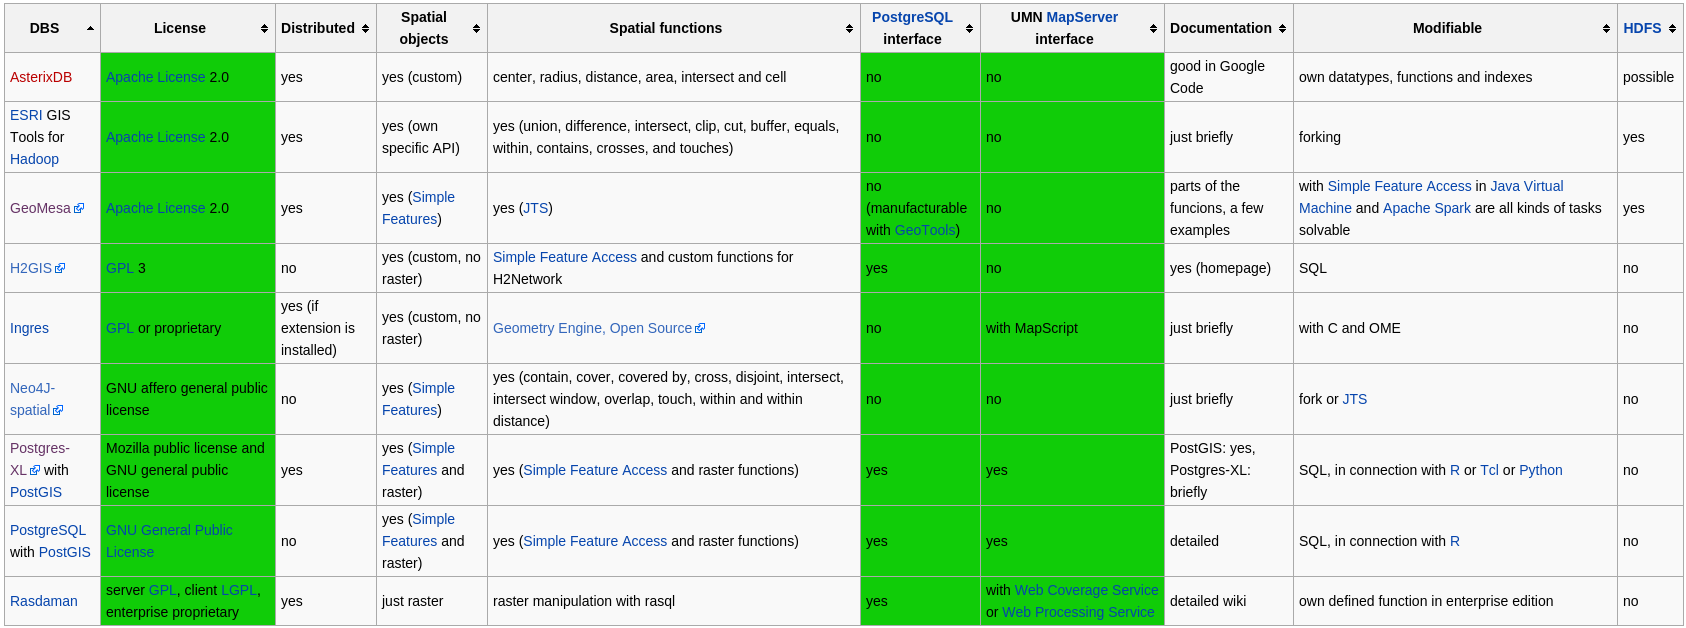
\includegraphics[width=1\hsize]{spatial_databases.png}
\caption{Relevante GIS nach Recherche}
\end{figure}
\begin{center}
\tiny
\url{https://en.wikipedia.org/wiki/Spatial_database}
\end{center}
%Auswahl nach Farbgebung
%Nutzwertanalyse mit Wichtung alle Metriken
\end{frame}

\begin{frame}\frametitle{Systemauswahl}

   \begin{columns}
    \begin{column}{.5\textwidth}
\ \ \ Nutzwert GeoMesa: 56
    \end{column}
    \begin{column}{.5\textwidth}
    
\includegraphics[width=.7\hsize]{geomesa.png}
    \end{column}
  \end{columns}
%https://raw.githubusercontent.com/geomesa/geomesa.github.io/master/img/geomesa-2x.png

\begin{table}
\begin{tabular}{|l|p{1.8cm}|l|p{1.9cm}|}
\hline
\textbf{Metrik} & \textbf{erreichter Wert} & \textbf{Erfüllung in \%} & \textbf{gewichteter Teilnutzen} \\ \hline
Interoperabilität & 7 & 58 & 17 \\ \hline
Funktionsumfang & 48 & 79 & 16 \\ \hline
Dokumentation & 4 & 31 & 11 \\ \hline
Modifizierbarkeit & 4 & 80 & 12 \\ \hline
\end{tabular}
\caption{Nutzwertanalyse GeoMesa}
\end{table}

\begin{center}
\tiny
\url{https://raw.githubusercontent.com/geomesa/geomesa.github.io/master/img/geomesa-2x.png}
\end{center}

\end{frame}

\begin{frame}\frametitle{Systemauswahl}

   \begin{columns}
    \begin{column}{.5\textwidth}
\ \ \ Nutzwert Postgres-XL: 86
    \end{column}
    \begin{column}{.5\textwidth}
    
\includegraphics[width=.45\hsize]{postgresxl.jpg}
    \end{column}
  \end{columns}
%http://www.postgres-xl.org/wp-content/uploads/2014/04/xl592x497g.jpg

\begin{table}
\begin{tabular}{|l|p{1.8cm}|l|p{1.9cm}|}
\hline
\textbf{Metrik} & \textbf{erreichter Wert} & \textbf{Erfüllung in \%} & \textbf{gewichteter Teilnutzen} \\ \hline
Interoperabilität & 12 & 100 & 30 \\ \hline
Funktionsumfang & 53 & 87 & 17 \\ \hline
Dokumentation & 9 & 69 & 24 \\ \hline
Modifizierbarkeit & 5 & 100 & 15 \\ \hline
\end{tabular}
\caption{Nutzwertanalyse Postgres-XL}
\end{table}

\begin{center}
\tiny
\url{http://www.postgres-xl.org/wp-content/uploads/2014/04/xl592x497g.jpg}
\end{center}

\end{frame}

\begin{frame}\frametitle{Systemauswahl}

   \begin{columns}
    \begin{column}{.5\textwidth}
\ \ \ Nutzwert Rasdaman: 51
    \end{column}
    \begin{column}{.5\textwidth}
    
\includegraphics[width=.6\hsize]{rasdaman.png}
    \end{column}
  \end{columns}
%http://www.faculty.jacobs-university.de/pbaumann/iu-bremen.de_pbaumann/Courses/InformationArchitecture/Rasdaman-doc/html/rasj/rasj/logo-rasdaman.gif

\begin{table}
\begin{tabular}{|l|p{1.8cm}|l|p{1.9cm}|}
\hline
\textbf{Metrik} & \textbf{erreichter Wert} & \textbf{Erfüllung in \%} & \textbf{gewichteter Teilnutzen} \\ \hline
Interoperabilität & 7 & 58 & 17 \\ \hline
Funktionsumfang & 10 & 16 & 3 \\ \hline
Dokumentation & 8 & 62 & 22 \\ \hline
Modifizierbarkeit & 3 & 60 & 9 \\ \hline
\end{tabular}
\caption{Nutzwertanalyse Rasdaman}
\end{table}

\begin{center}
\tiny
\url{http://www.rasdaman.org/chrome/site/trac_logo.png}
\end{center}

\end{frame}

\section{Untersuchung von Postgres-XL}
%Ausschnitt aus Thesis

%
\begin{frame}\frametitle{Untersuchung von Postgres-XL}

\begin{figure}
\centering
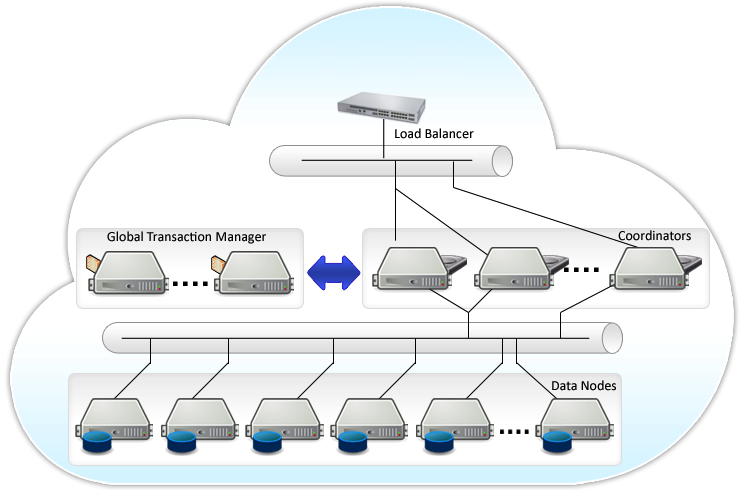
\includegraphics[width=1\hsize]{../Abbildungen/postgresxl-structure.jpg}
\caption{Aufbau von Postgres-XL}
\end{figure}
\end{frame}

\begin{frame}\frametitle{Untersuchung von Postgres-XL}
%Installation, Einrichtung
\begin{block}{Schnittstellen:}
Erfolgt analog zu PostgreSQL mit PostGIS mit Coordinator.
%Für SQL und UMN
\end{block}

\vspace{\baselineskip}
\vspace{\baselineskip}

\begin{block}{Verarbeitung:}
Abhängig der Verteilung der Daten sind ausgewählte Knoten aktiv.\\
Aufruf und Bibliotheken analog zu PostgreSQL mit PostGIS.
\end{block}

\end{frame}

\begin{frame}\frametitle{Untersuchung von Postgres-XL}


\end{frame}

\section{Tests}
%Ausschnitt aus Thesis

\section{Fazit}
%analog Thesis
 
\begin{frame}\frametitle{}


\end{frame}

\end{document}
